\section{Results}
\subsection{Determining stable spinodal compositions}
The Hessian of the demixing free energy is used to identify stable spinodal compositions. By analyzing the values of $\Delta F$, the range of chromium compositions where spinodal demixing is stable could be determined. This information is crucial for understanding the behavior of materials undergoing demixing processes and provides insights into their stability. Verifying phase transition indicators enable investigating properties to detect these phase transitions. 

Thermodynamics of demixing for body-centered cubic iron-chrome alloy calculated as a function of chromium composition. \cite{korzhavyi2009electronic,trochet2021influence,levesque2011simple, binder2001spinodal}(a) Enthalpy of demixing. (b) Entropy of demixing. (c) Free energy of demixing. 

Results from the Hessian matrix of the demixing free energy ($\Delta F$) show that for chromium compositions between 15\% and 45\%, the eigenvalues of the Hessian are negative, indicating that the system is within the spinodal region and thus unstable to demixing. Conversely, compositions outside this range displayed positive eigenvalues, suggesting that the alloy compositions are stable against spinodal decomposition.

\subsection{Obtaining elastic tensor from quantum mechanical calculations}
Quantum mechanical calculations provide a means to obtain the elastic tensor, a key parameter for characterizing material behavior. By employing thermoelastic equations derived from statistical mechanics, the elastic tensor could be determined from self-consistent field calculations for atomic positions from the electron density to gain insights into the elastodynamic properties of materials with lattice dynamic theory and other theoretical frameworks.

Elastic tensor from density functional theory calculations for body-centered cubic iron-chrome alloys as a function of chromium content. Stiffening is evident from increasing elastic constants with increasing chromium. \cite{korzhavyi2009electronic,razumovskiy2011first}

\subsubsection{Calculating elastic moduli and assessing embrittlement criteria}
Elastic moduli from quantum mechanical elastic tensor for body-centered cubic iron-chrome alloys as a function of chromium content. Stiffening is evident from increasing elastic moduli with increasing chromium. \cite{korzhavyi2009electronic,razumovskiy2011first}

The calculated elastic moduli, including Young's modulus, shear modulus, and bulk modulus, show a monotonically increasing trend with the addition of chromium content up to 30\%. Beyond this concentration, the rate of increase in moduli diminishes, indicating possible saturation in stiffening effect due to chromium addition.

\subsection{Predicting plastic embrittlement through quantum elastodynamics}
Quantum elastodynamics offers a means to predict plastic embrittlement in materials. By correlating the increase in elastic moduli with embrittlement tendency, it is possible to predict the embrittlement threshold for body-centered cubic iron-chrome alloys. The embrittlement criterion is assessed by the onset of a significant deviation from linearity in the plot of the elastic moduli versus chromium content.

The analysis shows that embrittlement becomes significant at chromium contents higher than 25\%, where the increase in elastic moduli starts to plateau. This plateau corresponds with an increase in the brittleness index, implying that alloys with chromium content above this threshold may be more prone to plastic embrittlement. This finding suggests that the control of chromium content is critical in designing iron-chrome alloys with optimized balance between stiffness and ductility.


\begin{figure}[!ht]
	\centering
	\begin{subfigure}{0.9\textwidth}
         \centering
         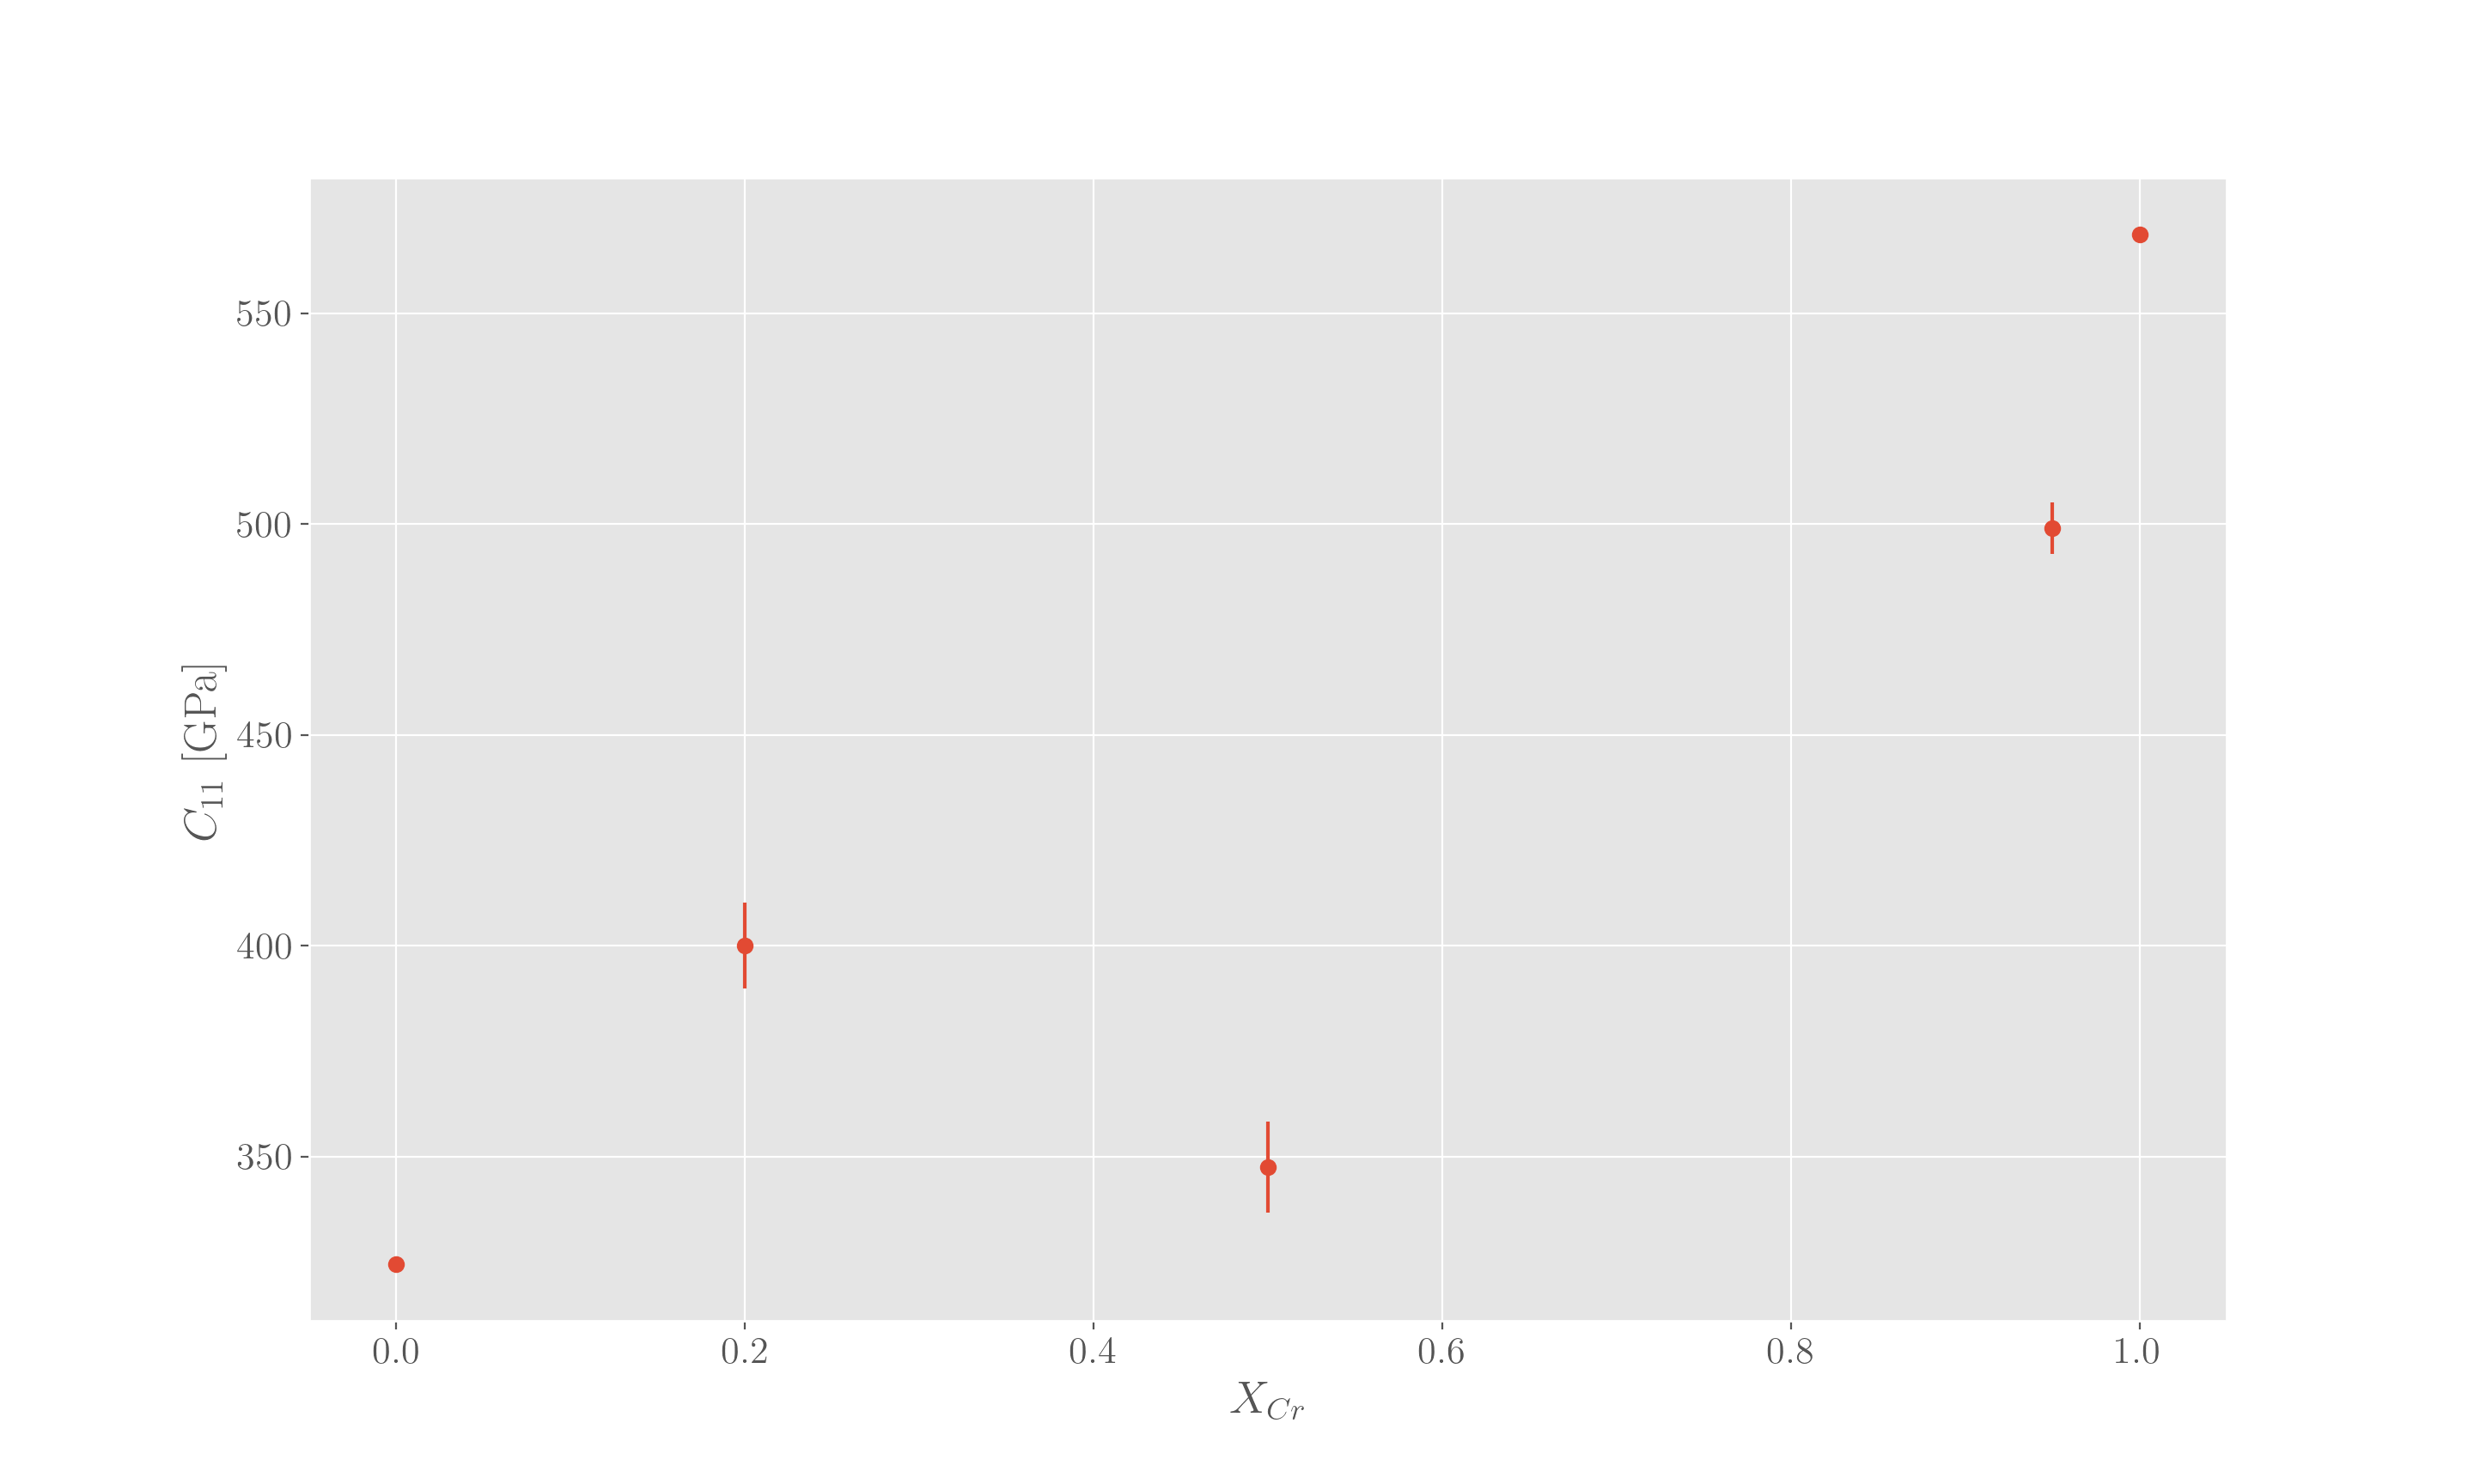
\includegraphics[width=\linewidth]{Parts/Figures/C11.png}
         \caption{Normal constant, \(C_{11}\), illustrating the longitudinal stiffness of bcc binary FeCr alloy as a function of chromium composition. This stiffness parameter is crucial for understanding the acoustic velocity and mechanical properties of the material.}
         \label{fig1a}
     \end{subfigure}
     \hfill
     \begin{subfigure}{0.45\textwidth}
         \centering
         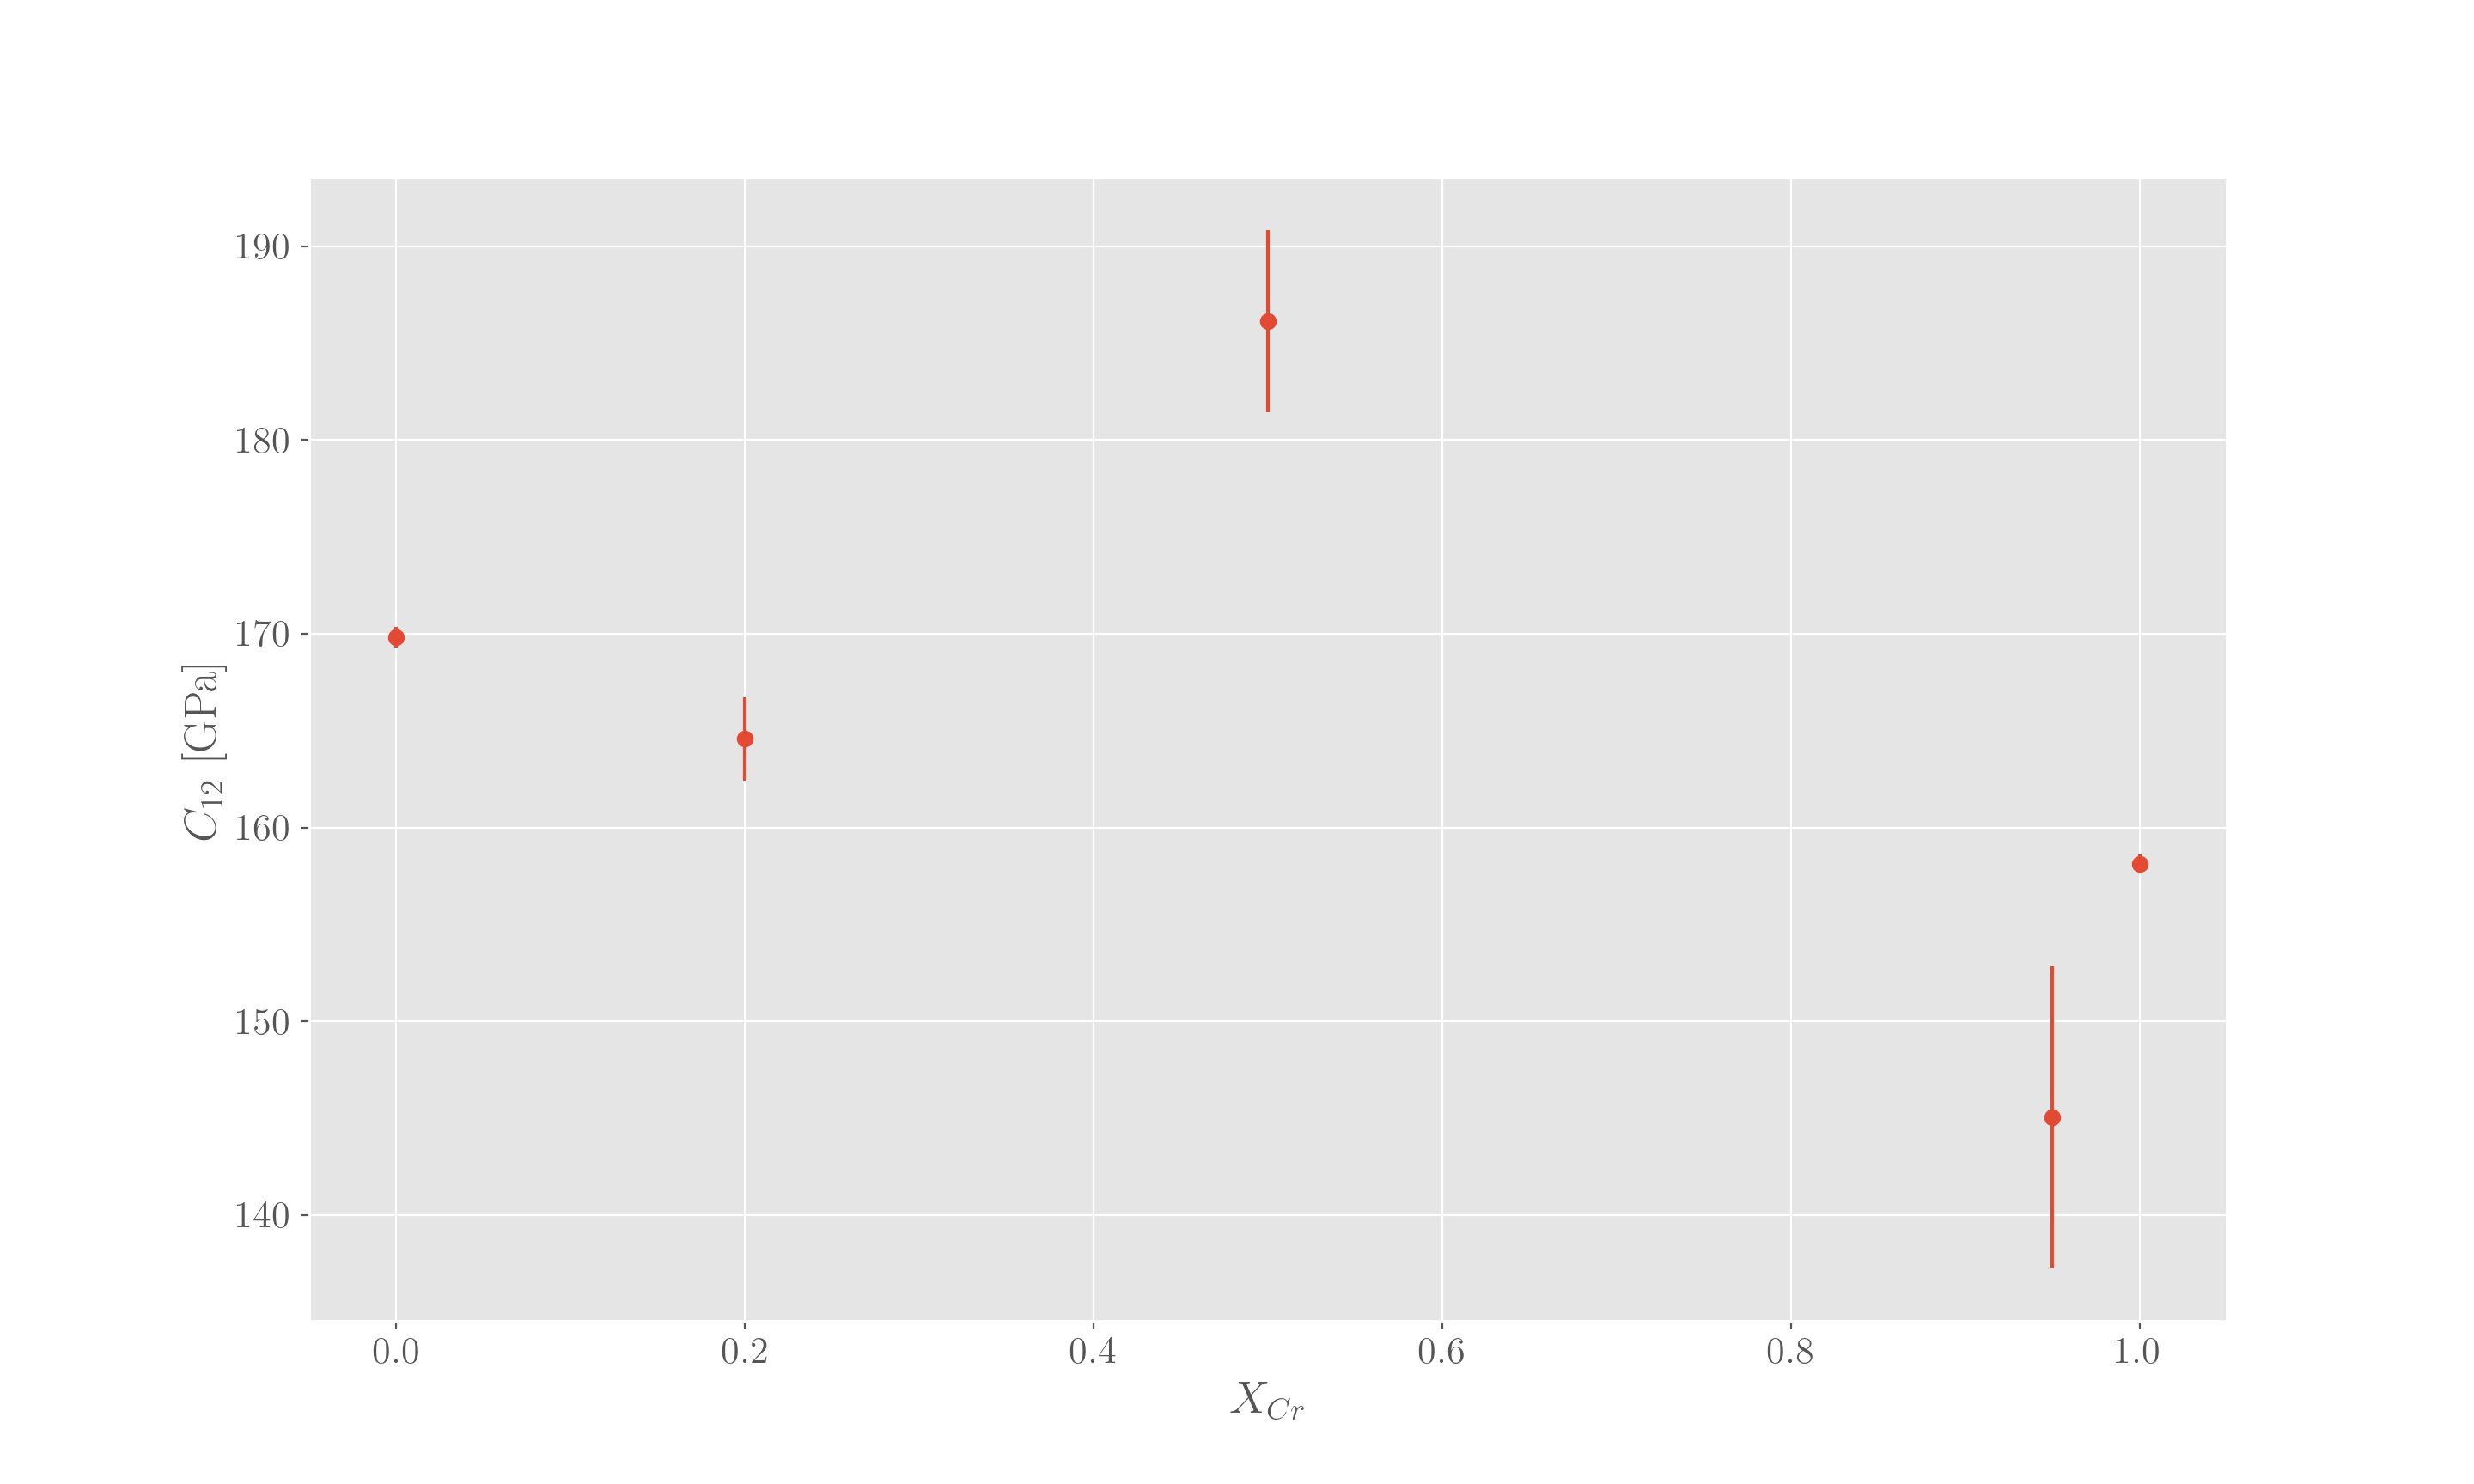
\includegraphics[width=\linewidth]{Parts/Figures/C12.png}
         \caption{The interplanar elastic constant \(C_{12}\), showing the coupling between axial and lateral strains, indicative of the alloy's resistance to shear along crystallographic planes.}
         \label{fig1b}
     \end{subfigure}
     \hfill
     \begin{subfigure}{0.45\textwidth}
         \centering
         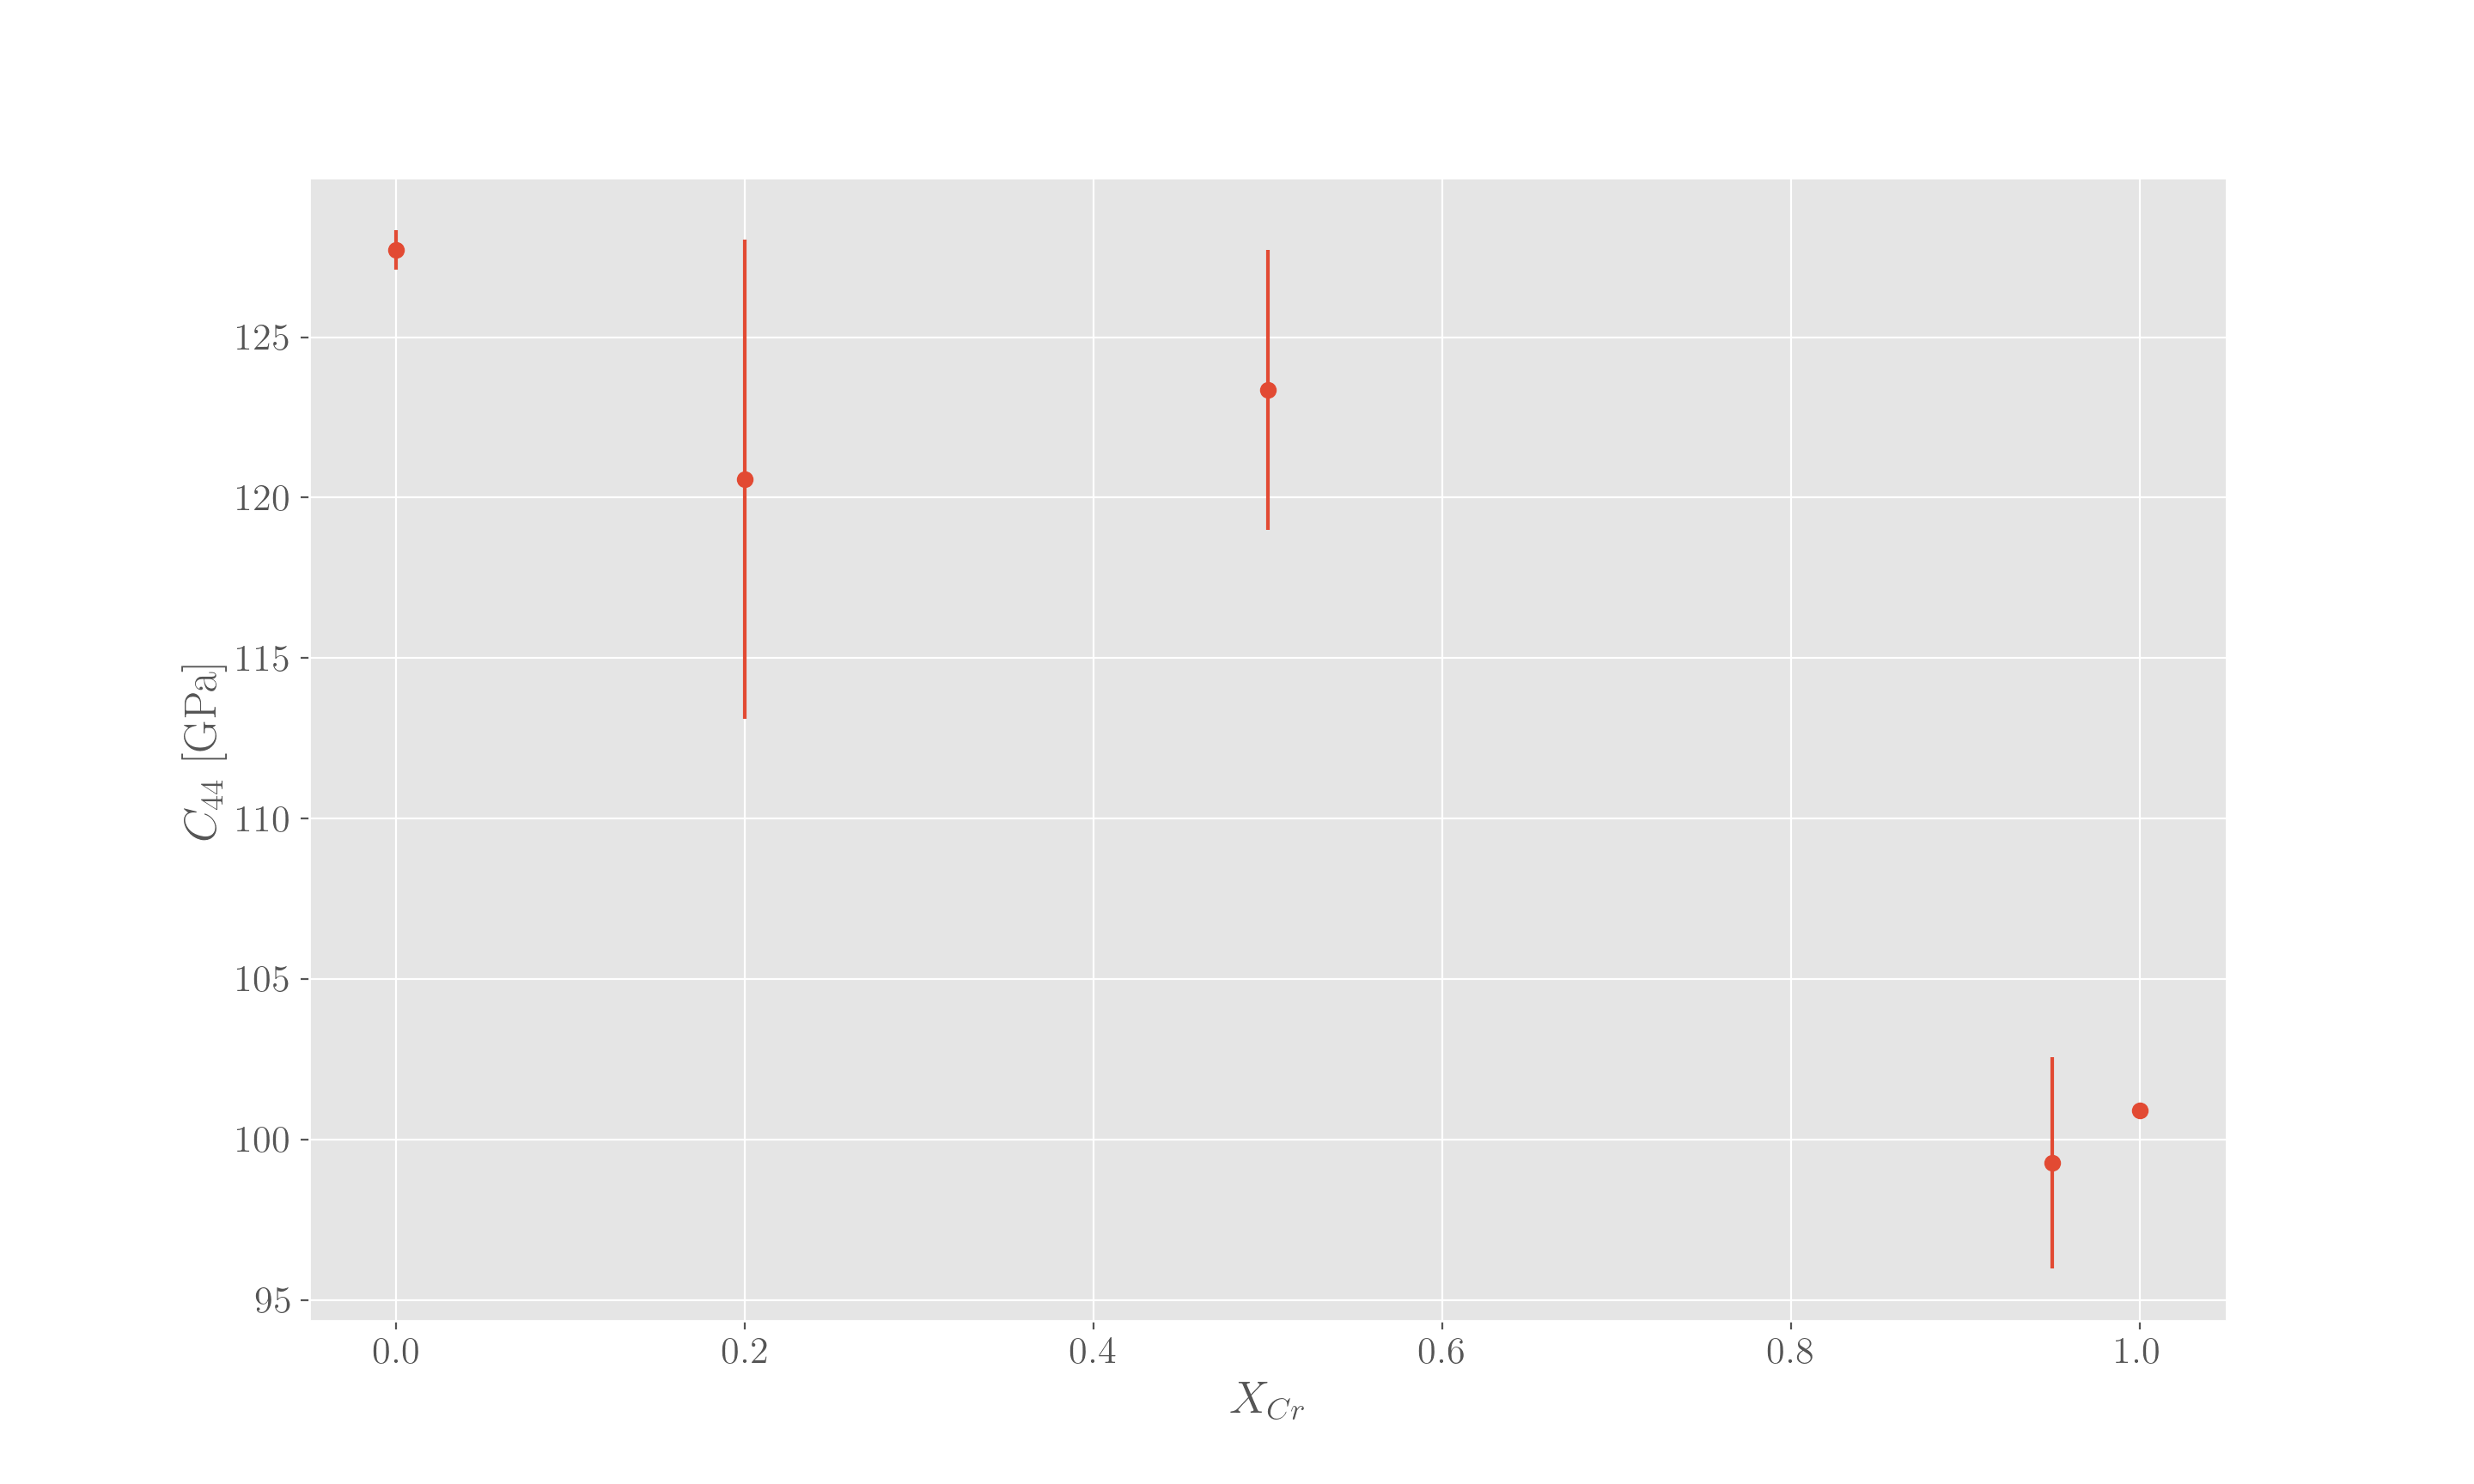
\includegraphics[width=\linewidth]{Parts/Figures/C44.png}
         \caption{Shear constant, \(C_{44}\), representing shear stiffness against deformation without volume change, critical for assessing material's resistance to applied shear stress.}
         \label{fig1c}
     \end{subfigure}
	\caption{Elastic constants of bcc binary FeCr as a function of Cr composition indicate spinodal decomposition-induced stiffening towards embrittlement. The trends and values are consistent with theoretical and experimental results reported in literature. (a) Shows the longitudinal stiffness parameter \(C_{11}\), important for evaluating the material's response to compressive and tensile stresses. (b) Highlights \(C_{12}\), which is essential for understanding the coupling between different types of strain. (c) Details \(C_{44}\), crucial for evaluating the shear deformation behavior.}
	\label{fig1}
\end{figure}


\begin{figure}[!ht]
	\centering
	\begin{subfigure}{0.9\textwidth}
         \centering
         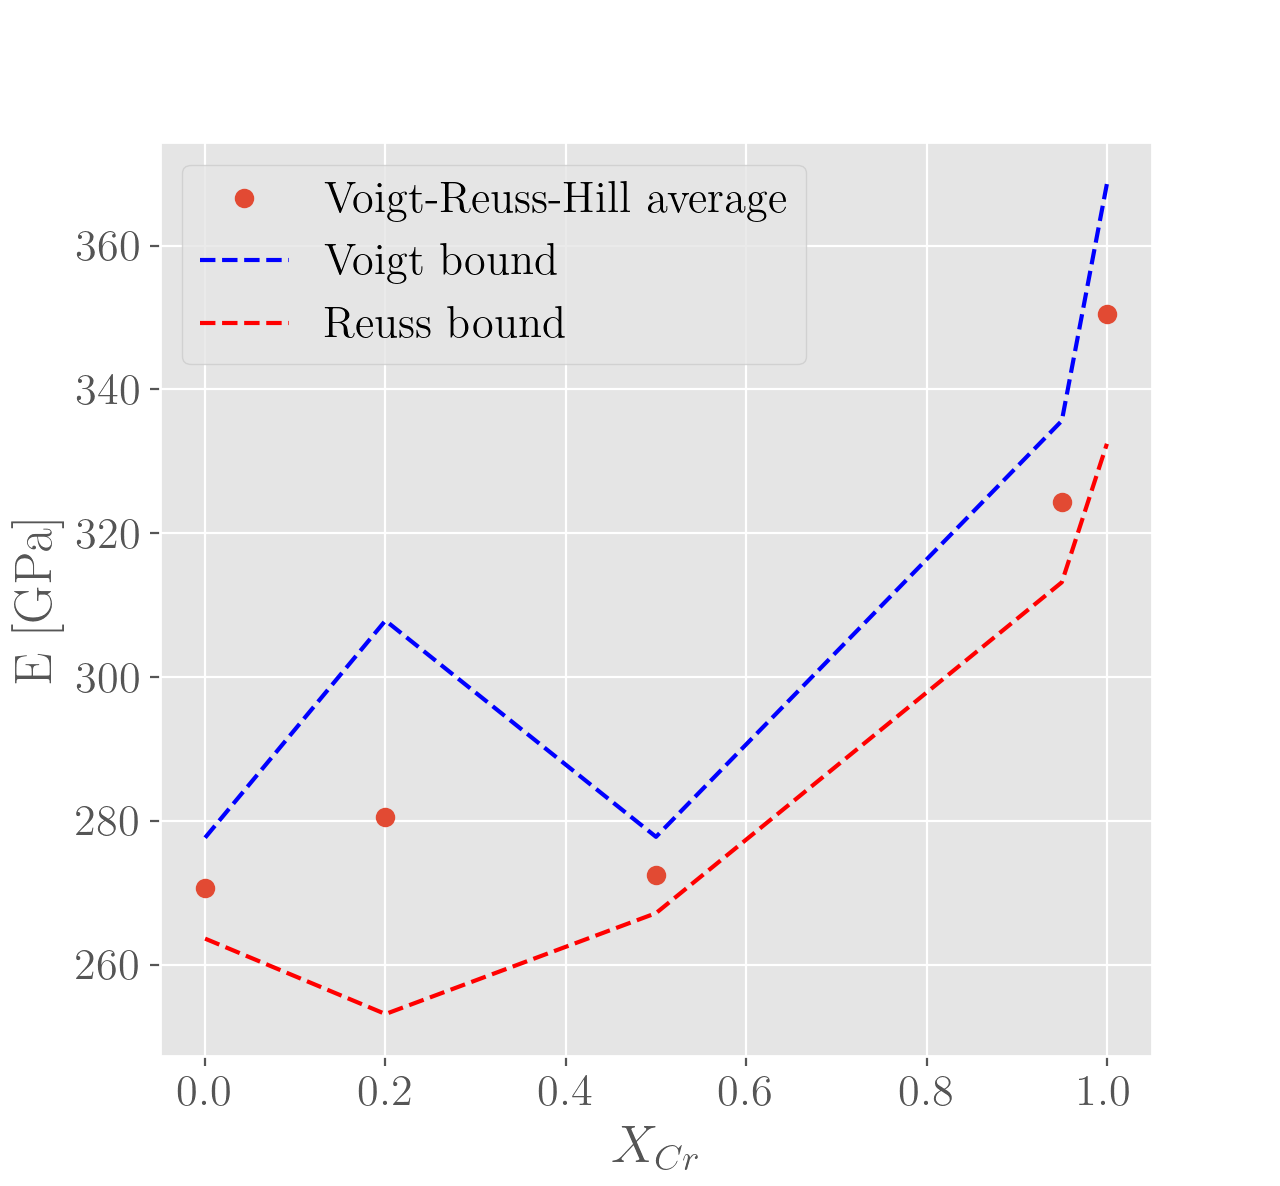
\includegraphics[width=\linewidth]{Parts/Figures/E_VRH.png}
         \caption{Elastic (Young's) Modulus, \(E_{VRH}\), indicating the material's stiffness and its ability to resist deformation under tensile stress.}
         \label{fig2a}
     \end{subfigure}
     \hfill
     \begin{subfigure}{0.45\textwidth}
         \centering
         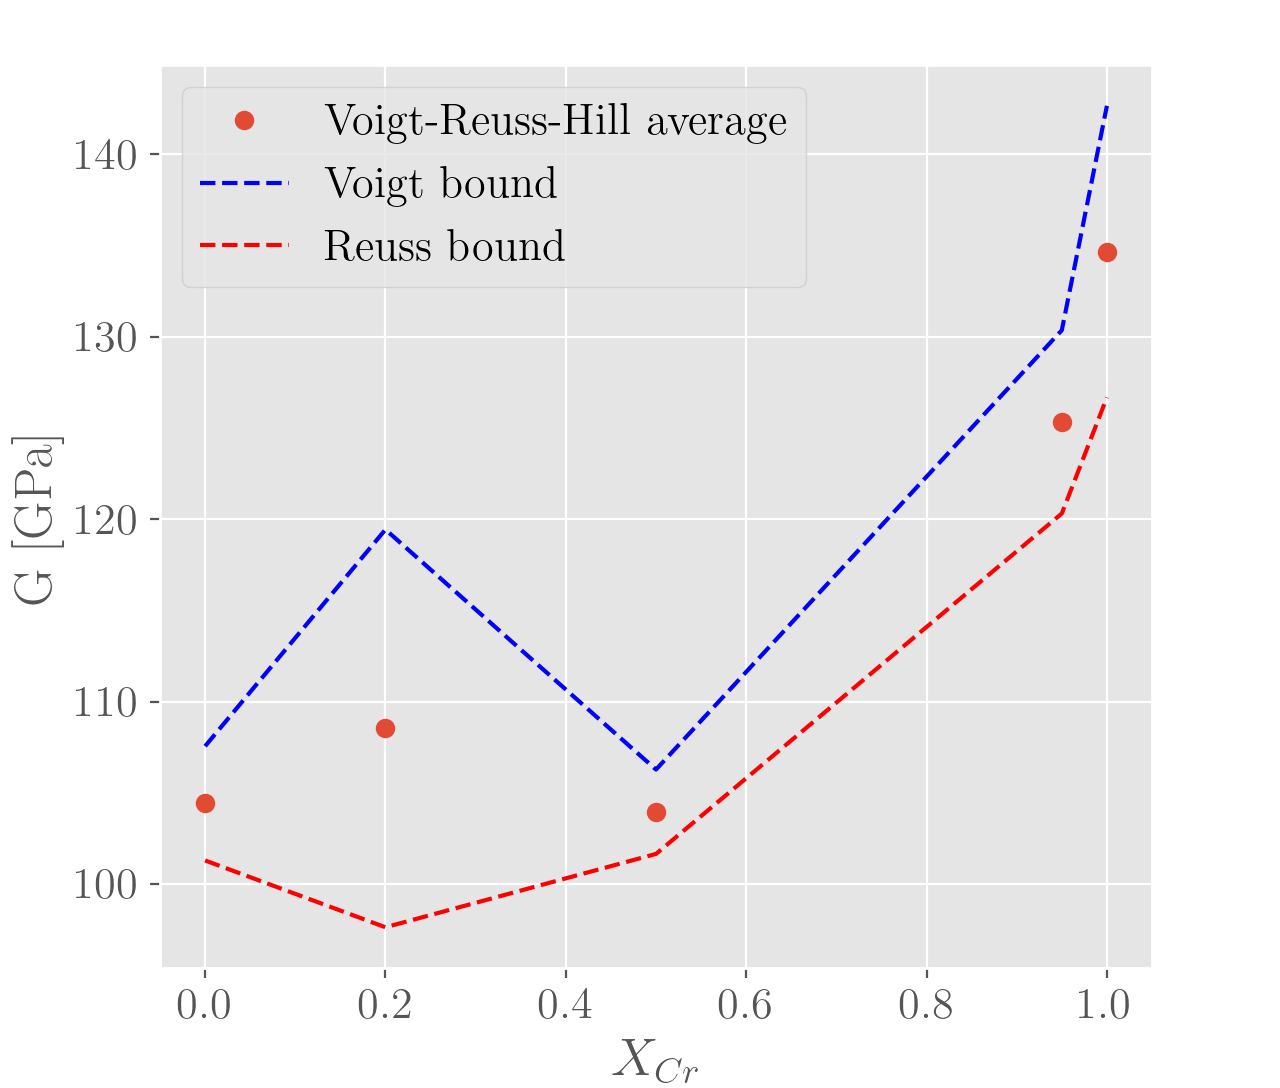
\includegraphics[width=\linewidth]{Parts/Figures/G_VRH.png}
         \caption{Shear modulus, \(G_{VRH}\), reflecting the material's ability to withstand shear deformation.}
         \label{fig2b}
     \end{subfigure}
     \hfill
     \begin{subfigure}{0.45\textwidth}
         \centering
         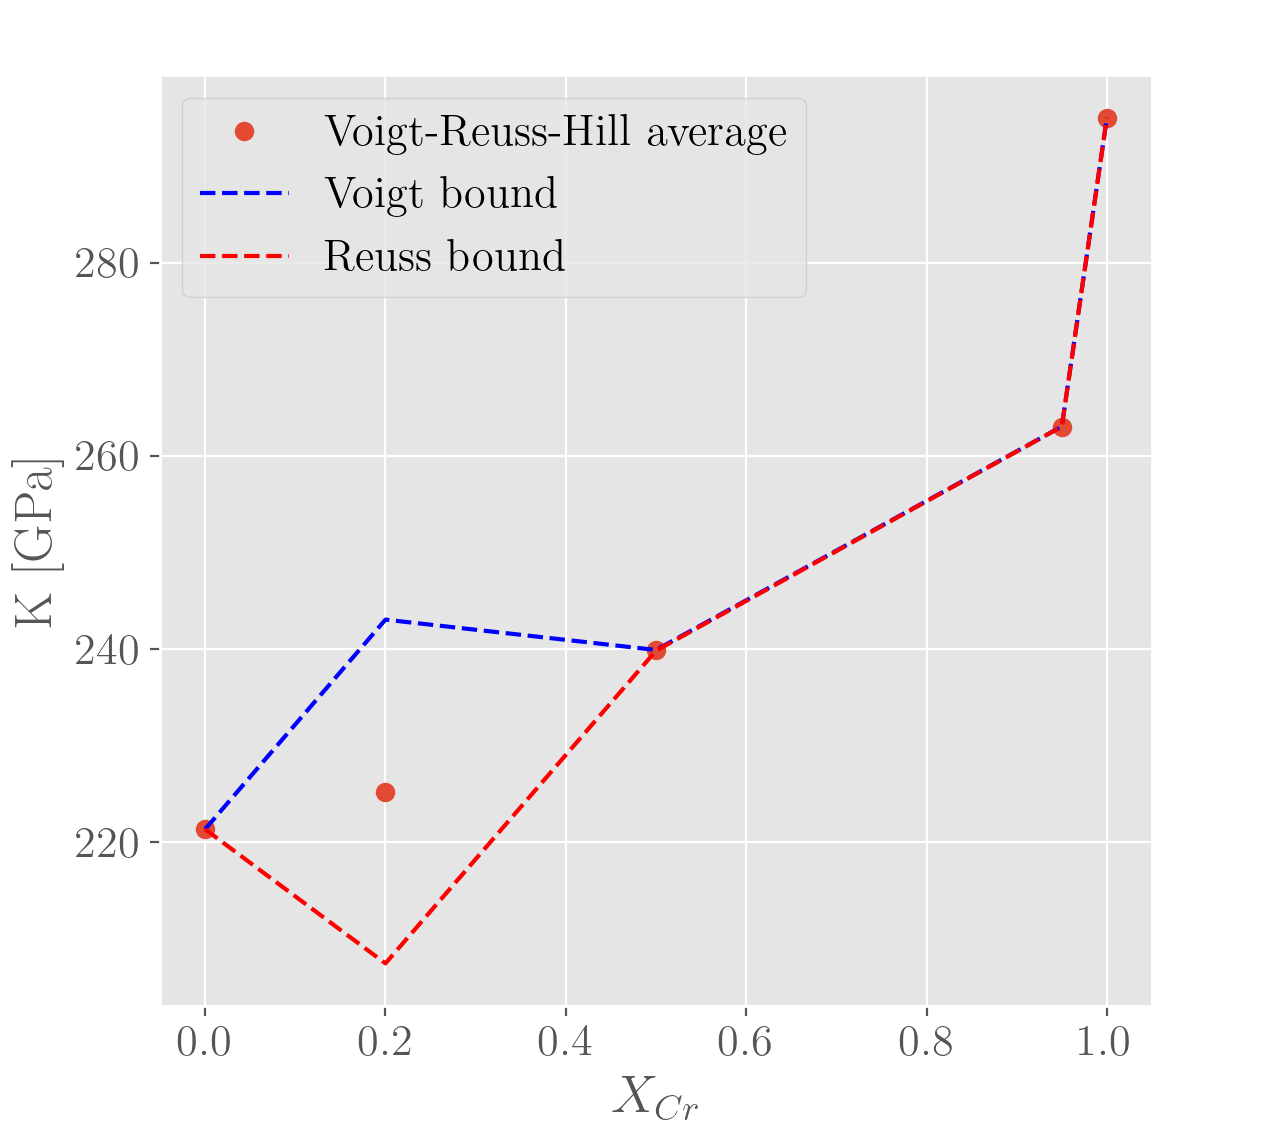
\includegraphics[width=\linewidth]{Parts/Figures/K_VRH.png}
         \caption{Bulk modulus, \(K_{VRH}\), which measures the material's resistance to uniform compression.}
         \label{fig2c}
     \end{subfigure}
	\caption{Elastic moduli of bcc binary FeCr as a function of Cr composition indicate spinodal decomposition-induced stiffening towards embrittlement. The trends and values are consistent with theoretical and experimental results reported in literature. (a) Elastic (Young's) Modulus demonstrates the material's overall stiffness. (b) Shear modulus is a measure of the alloy's rigidity against shear forces. (c) Bulk modulus assesses the material's compressibility under uniform pressure.}
	\label{fig2}
\end{figure}

\begin{sidewaysfigure}[!ht]
	\centering
	\begin{subfigure}{0.7\textwidth}
         \centering
         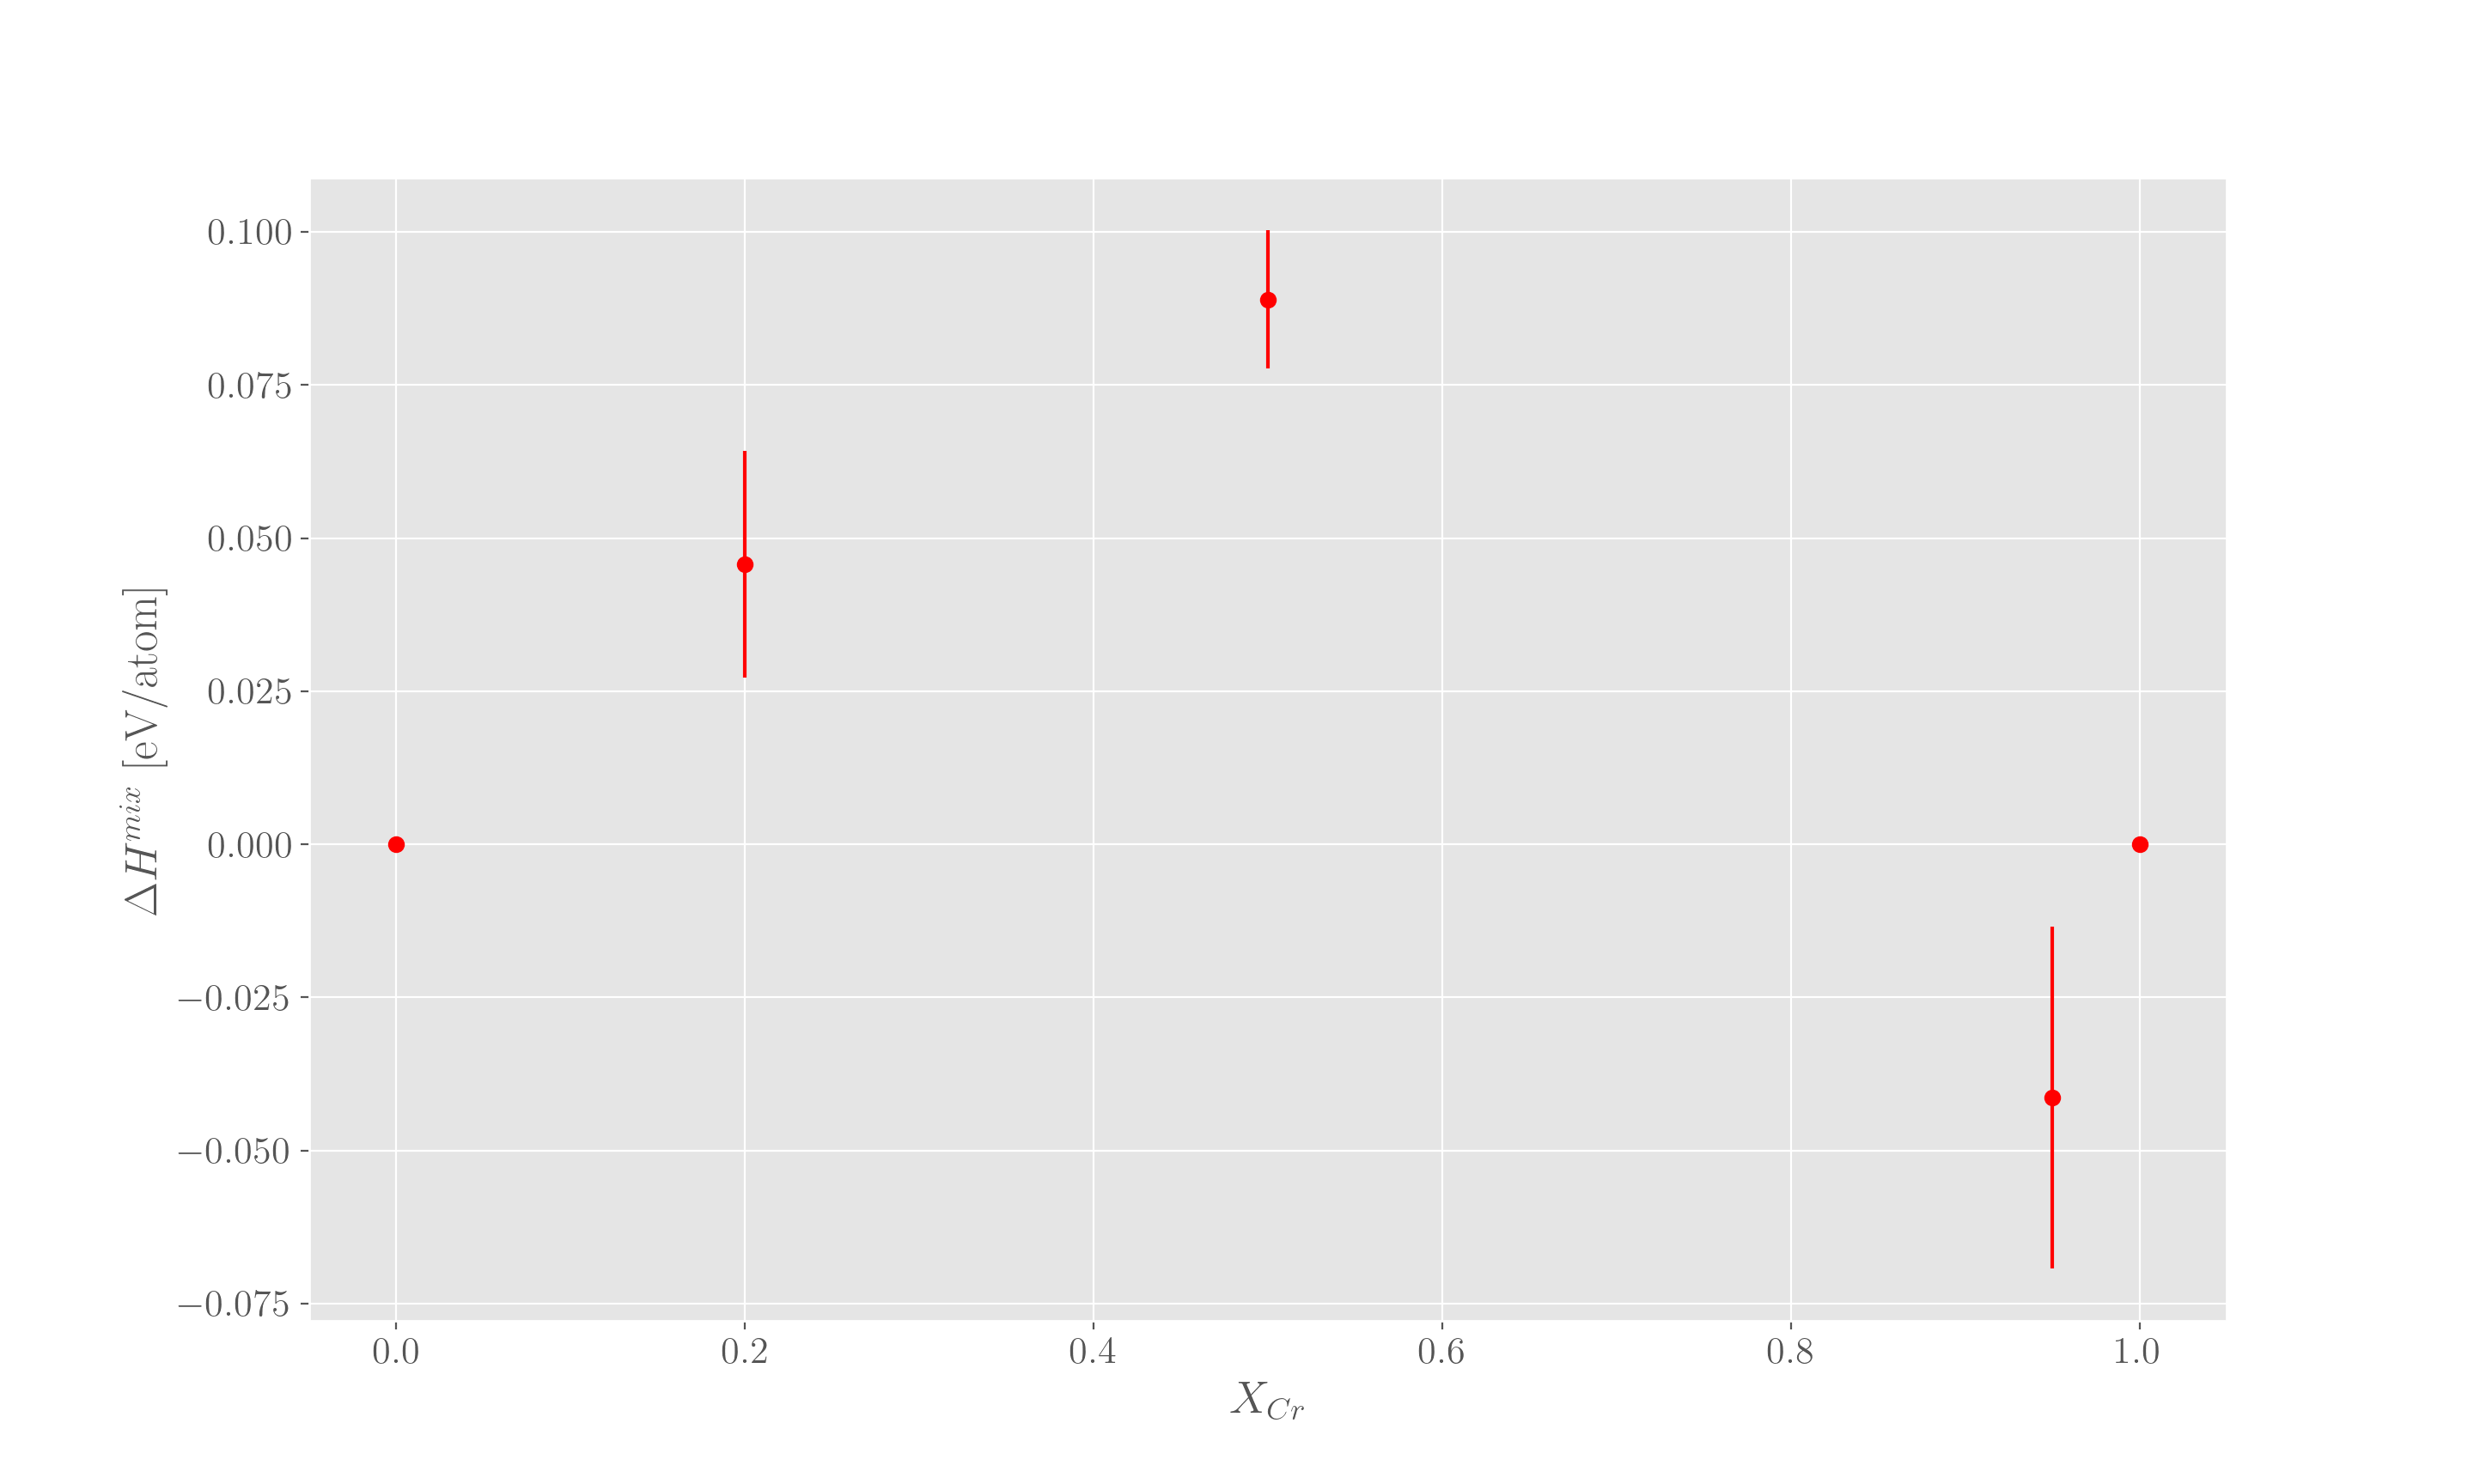
\includegraphics[width=\linewidth]{Parts/Figures/Hmix-vF.png}
         \caption{Enthalpy of mixing, showing the thermodynamic favorability of phase separation in bcc $\delta$-ferrite in cast austenitic stainless steels through spinodal decomposition.}
         \label{fig3a}
     \end{subfigure}
     \begin{subfigure}{0.3\textwidth}
         \centering
         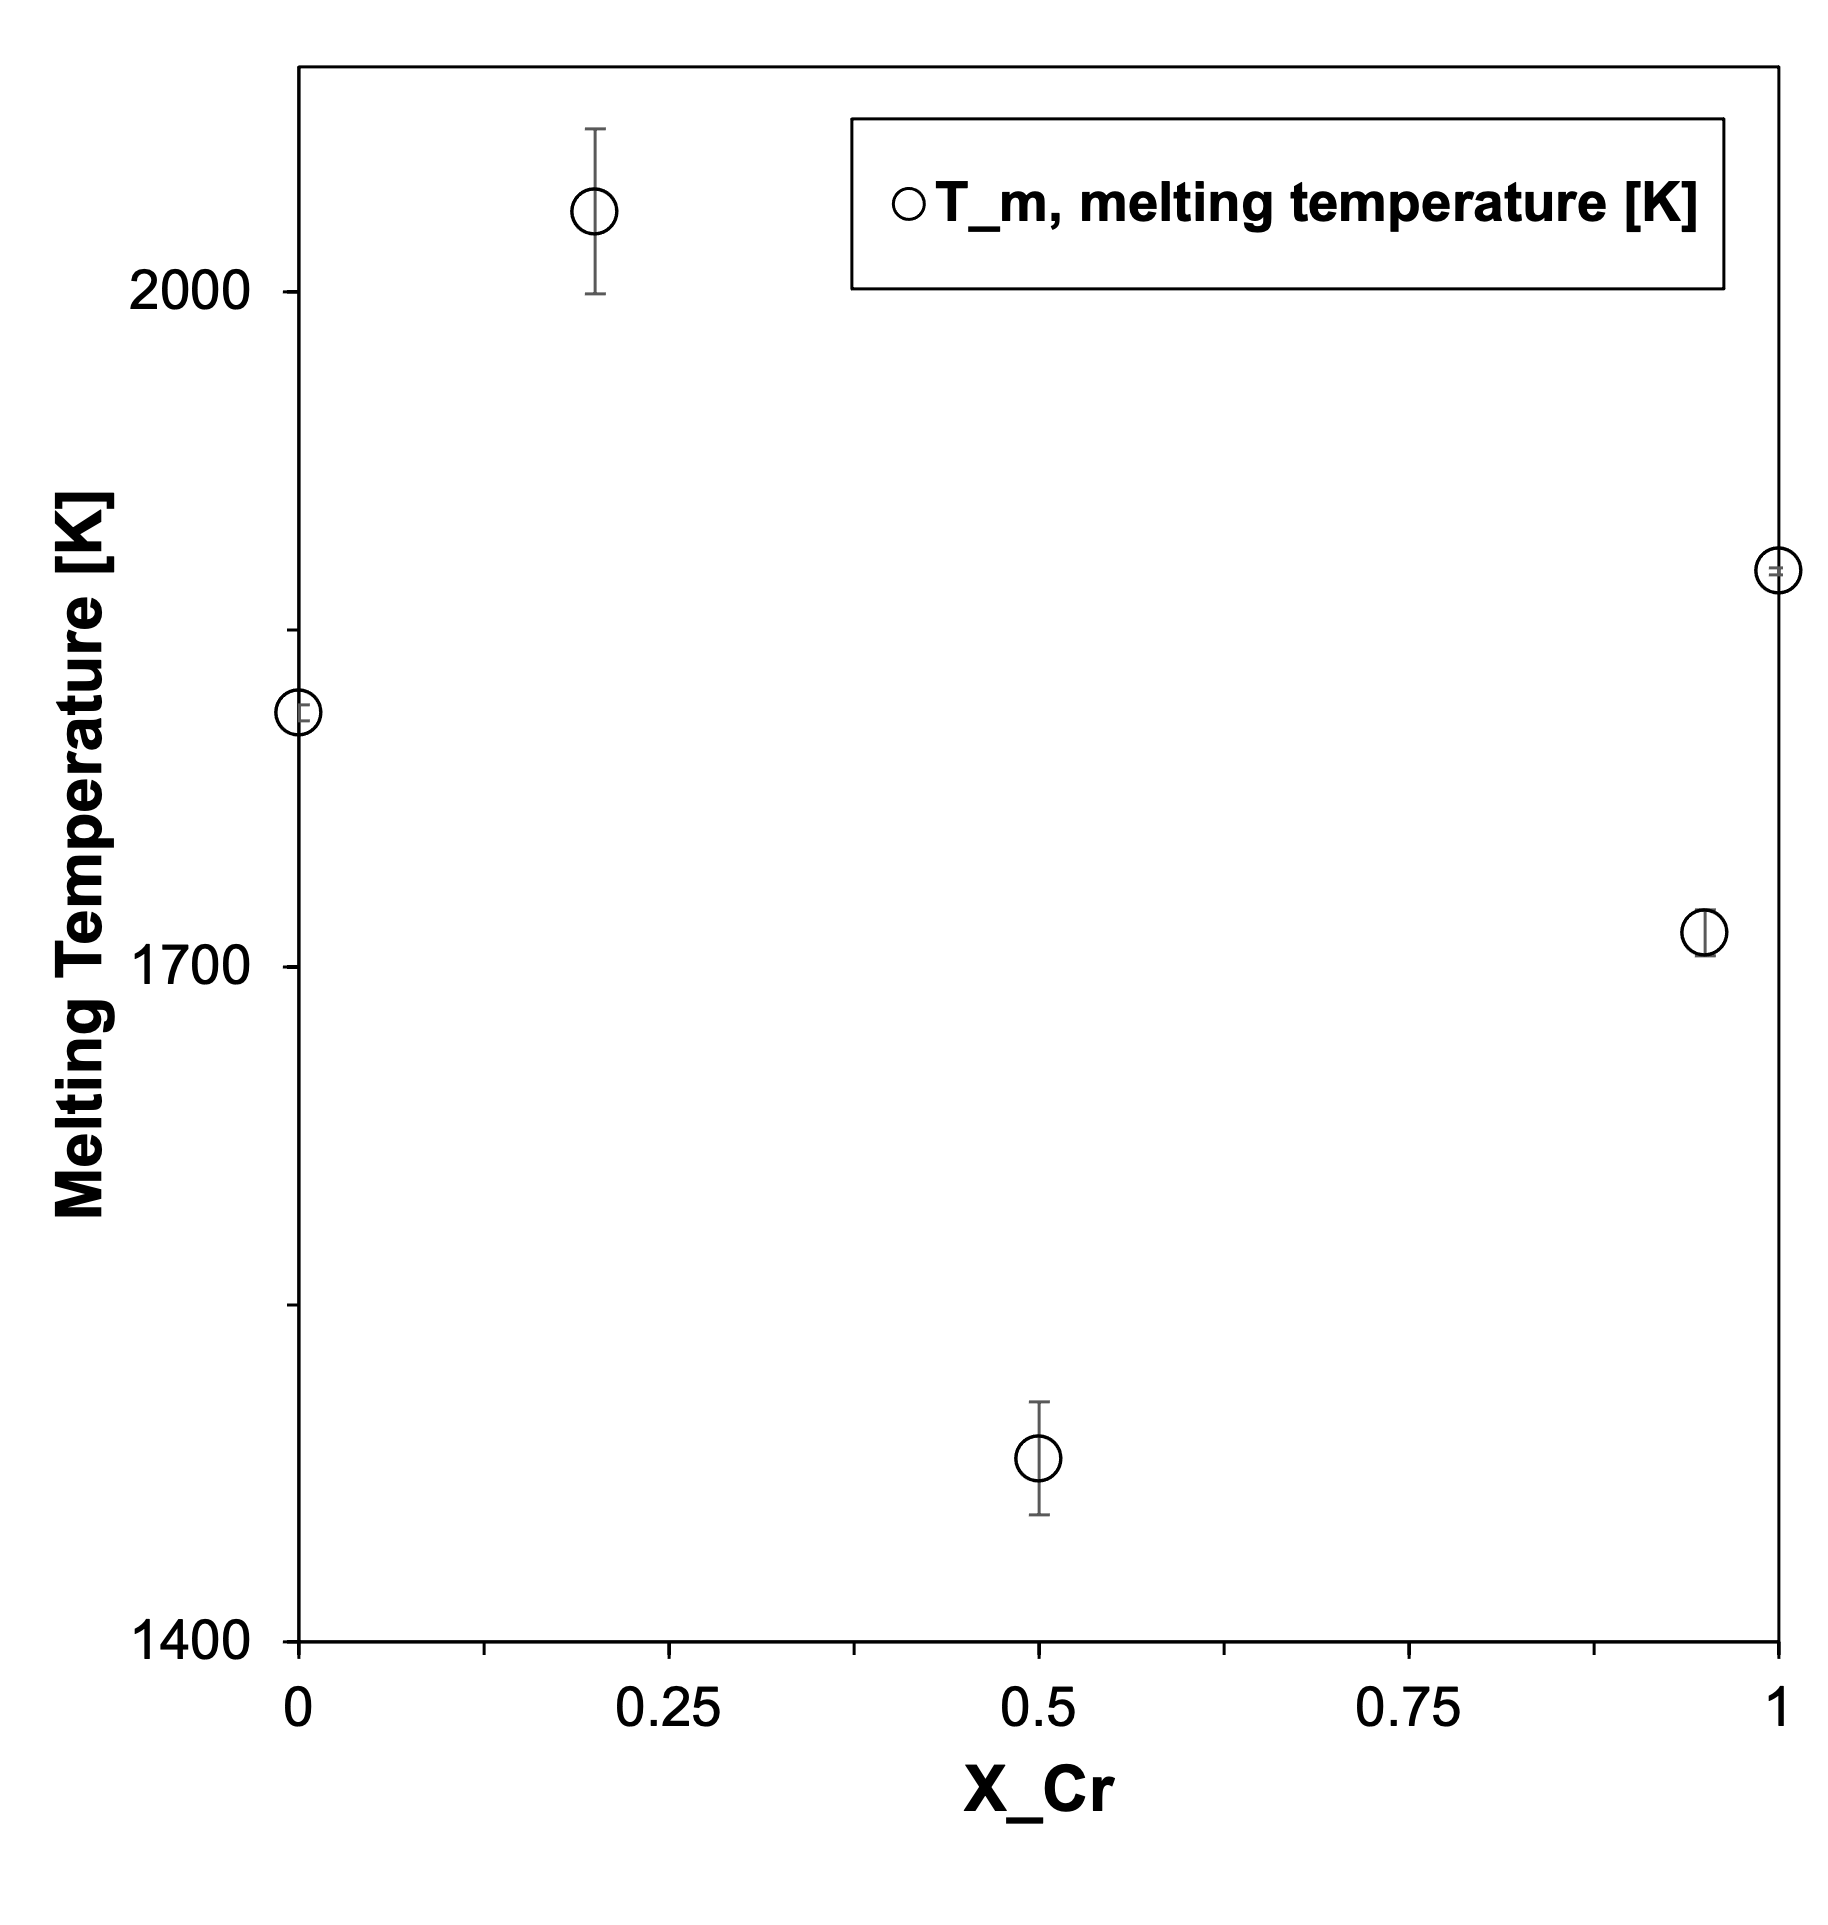
\includegraphics[width=\linewidth]{Parts/Figures/TMvsX_v2.png}
         \caption{\(T_M\), melting temperature, indicating how the thermal stability of the material changes with Cr composition.}
         \label{fig3b}
     \end{subfigure}
     \begin{subfigure}{0.3\textwidth}
         \centering
         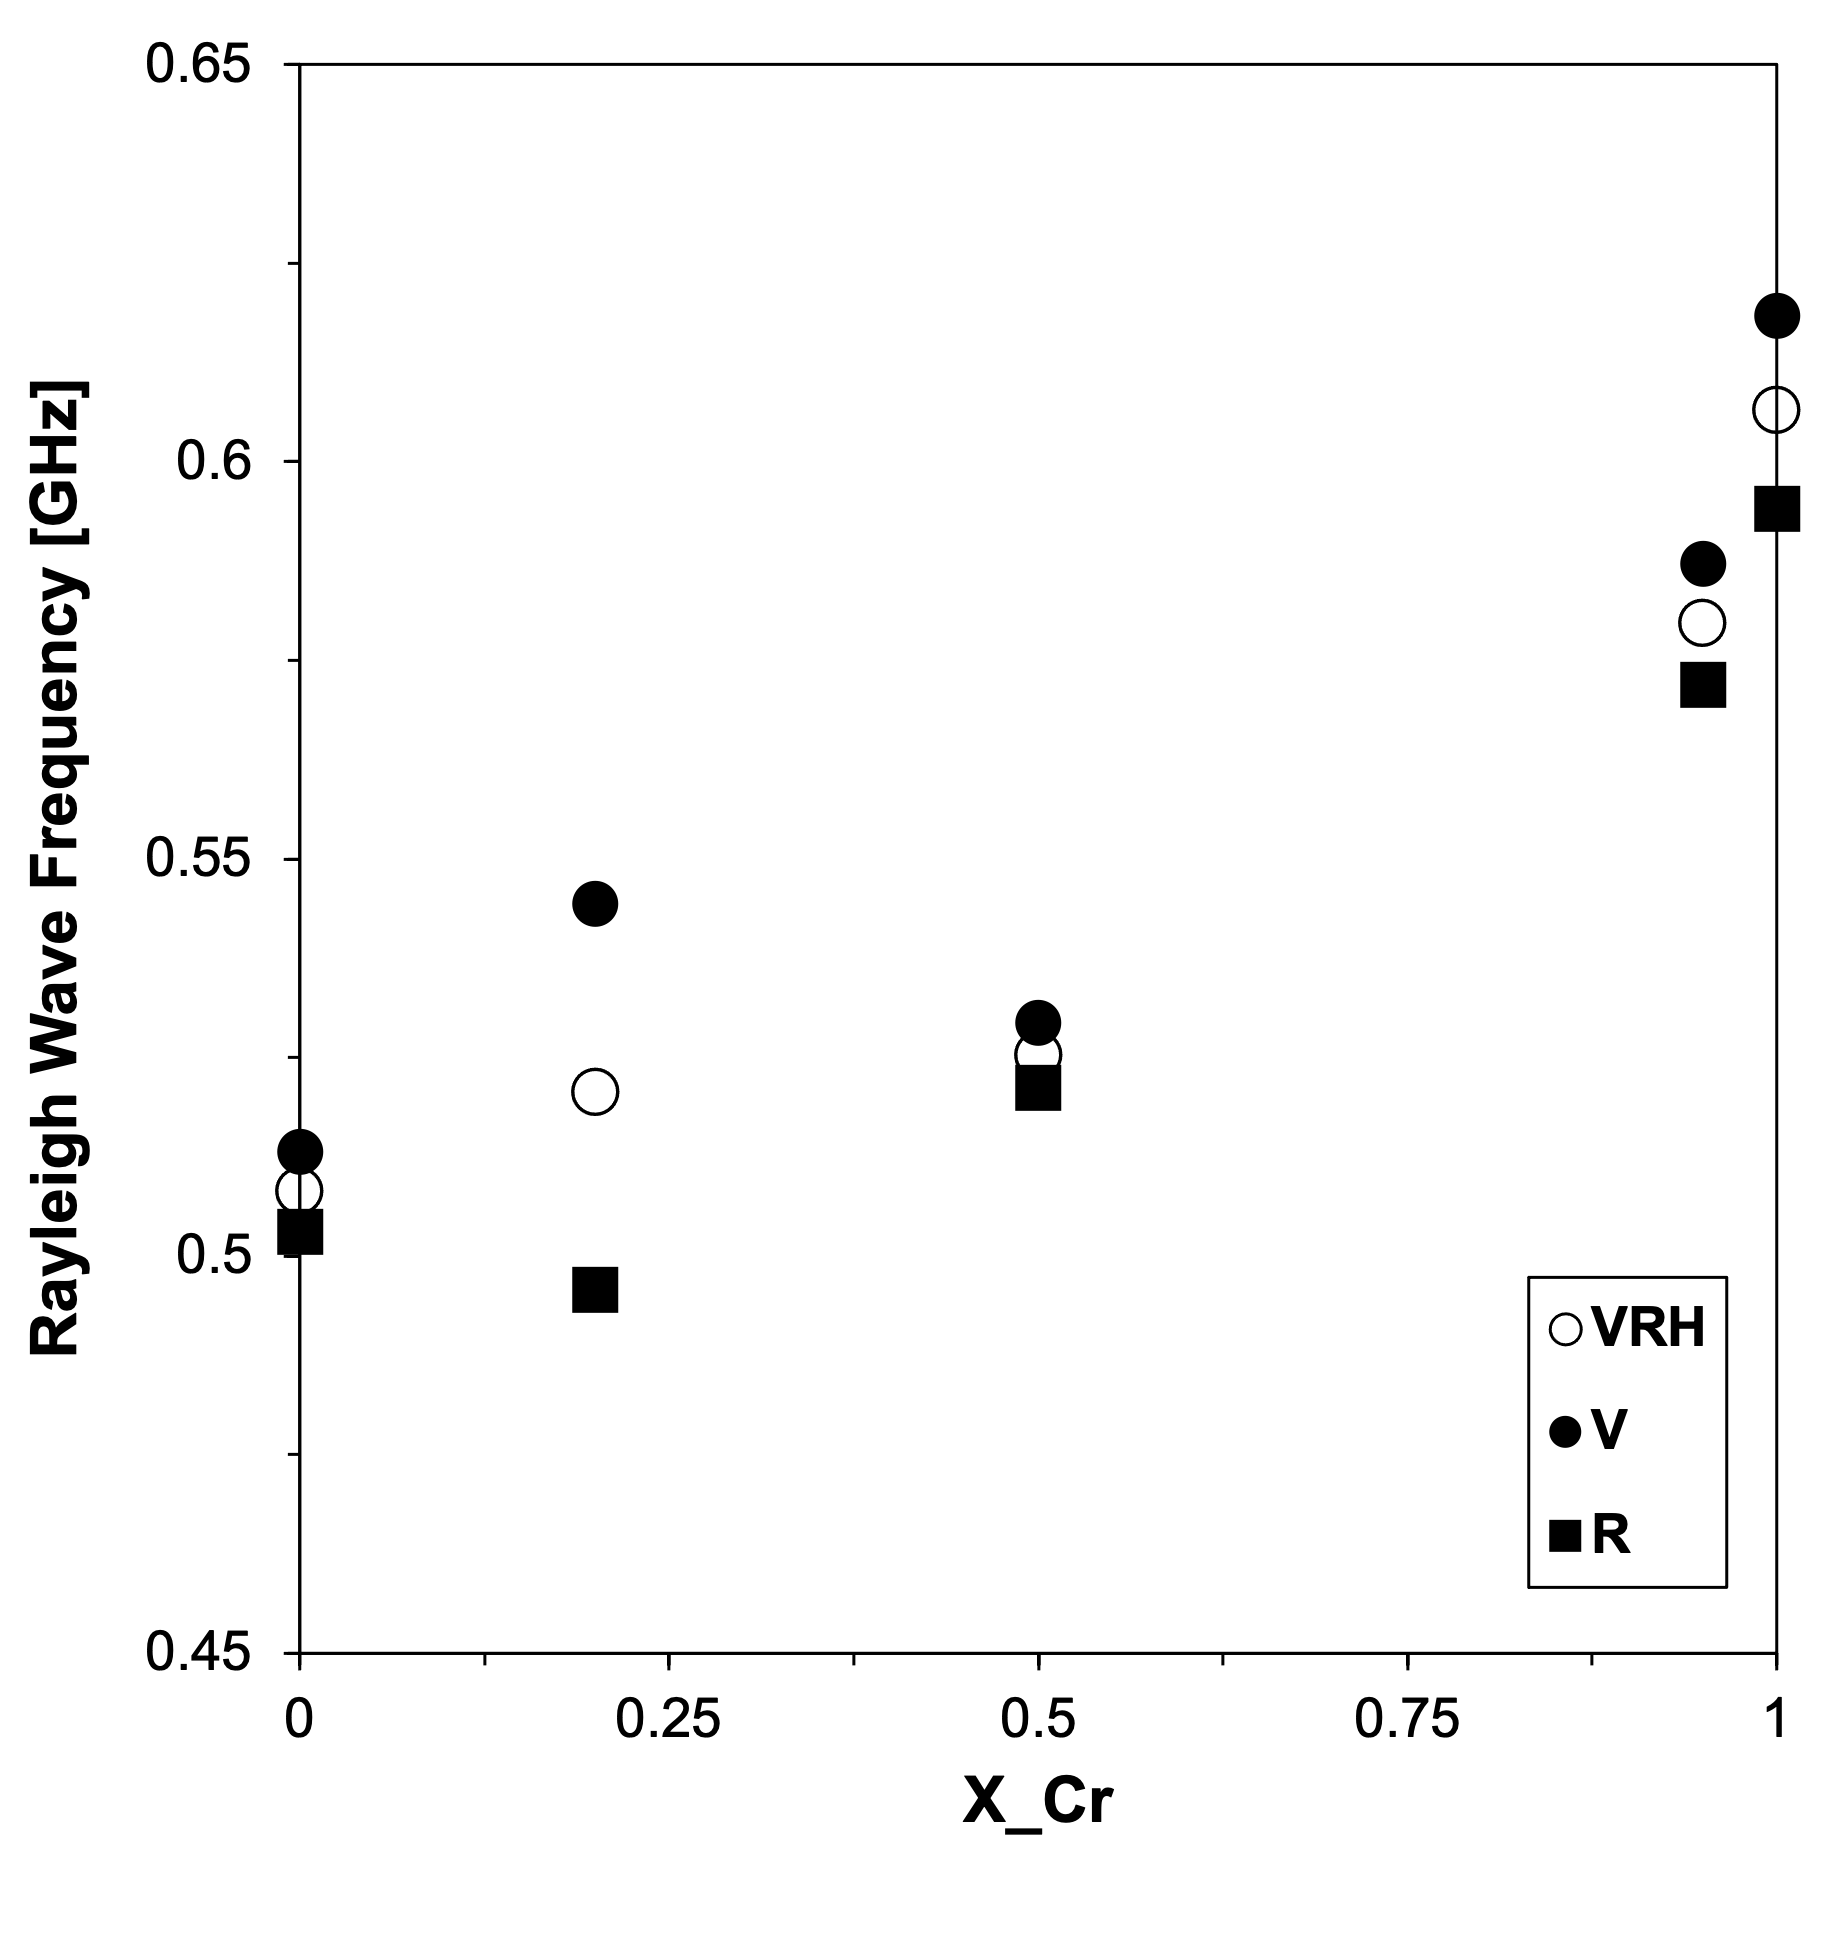
\includegraphics[width=\linewidth]{Parts/Figures/f_rwVsX_vF.png}
         \caption{Rayleigh wave frequencies, illustrating the impact of spinodal decomposition on the material's surface acoustic properties.}
         \label{fig3c}
     \end{subfigure}
     \begin{subfigure}{0.3\textwidth}
         \centering
         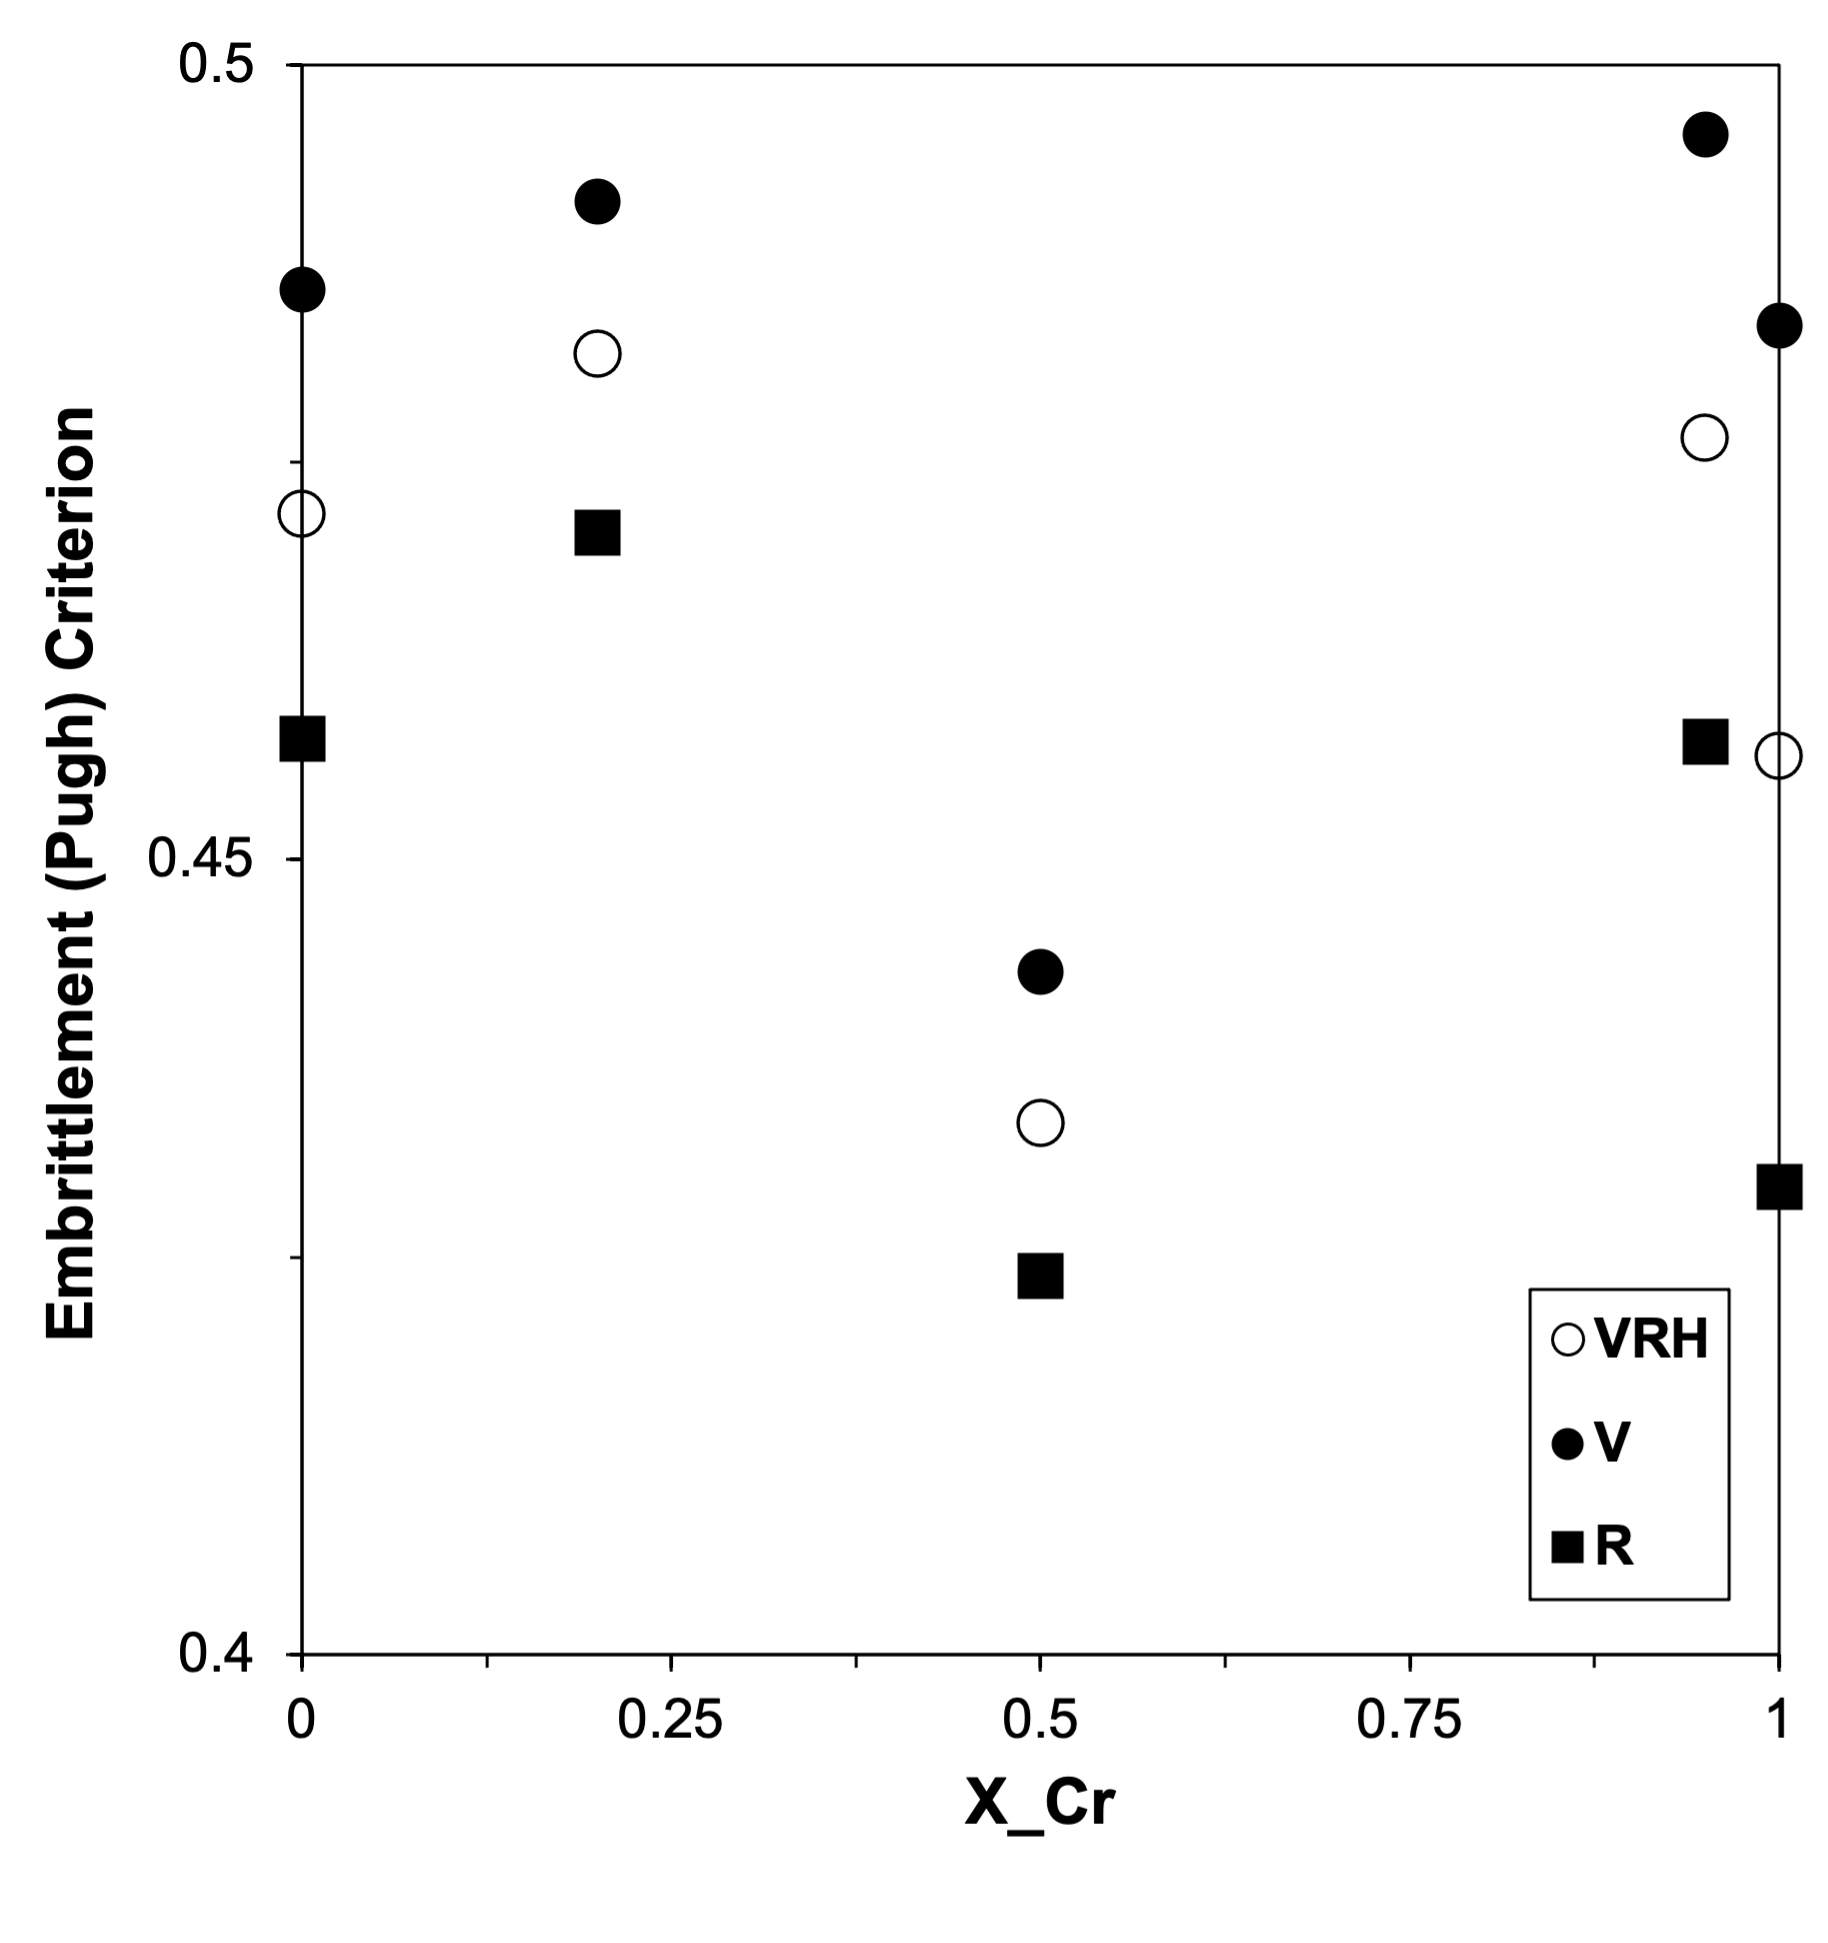
\includegraphics[width=\linewidth]{Parts/Figures/EvsX_vF.png}
         \caption{Embrittlement (Pugh) Criterion, calculated to evaluate the embrittlement risk associated with varying Cr compositions.}
         \label{fig3d}
     \end{subfigure}
	\caption{(a) The enthalpy of mixing demonstrates the thermodynamic drive towards phase separation indicative of spinodal decomposition, affecting the material's mechanical integrity. (b) Variations in the melting temperature as a function of Cr composition offer insights into the thermal stability and potential phase transformations within the alloy. (c) Changes in Rayleigh wave frequencies across compositions highlight alterations in surface acoustic properties, correlating with mechanical behavior. (d) The Embrittlement (Pugh) Criterion allows for assessing the risk of material embrittlement due to changes in composition, crucial for ensuring material reliability in critical applications.}
	\label{fig3}
\end{sidewaysfigure}


\begin{sidewaysfigure}[!ht]
    \centering
    \begin{subfigure}{0.9\textwidth}
        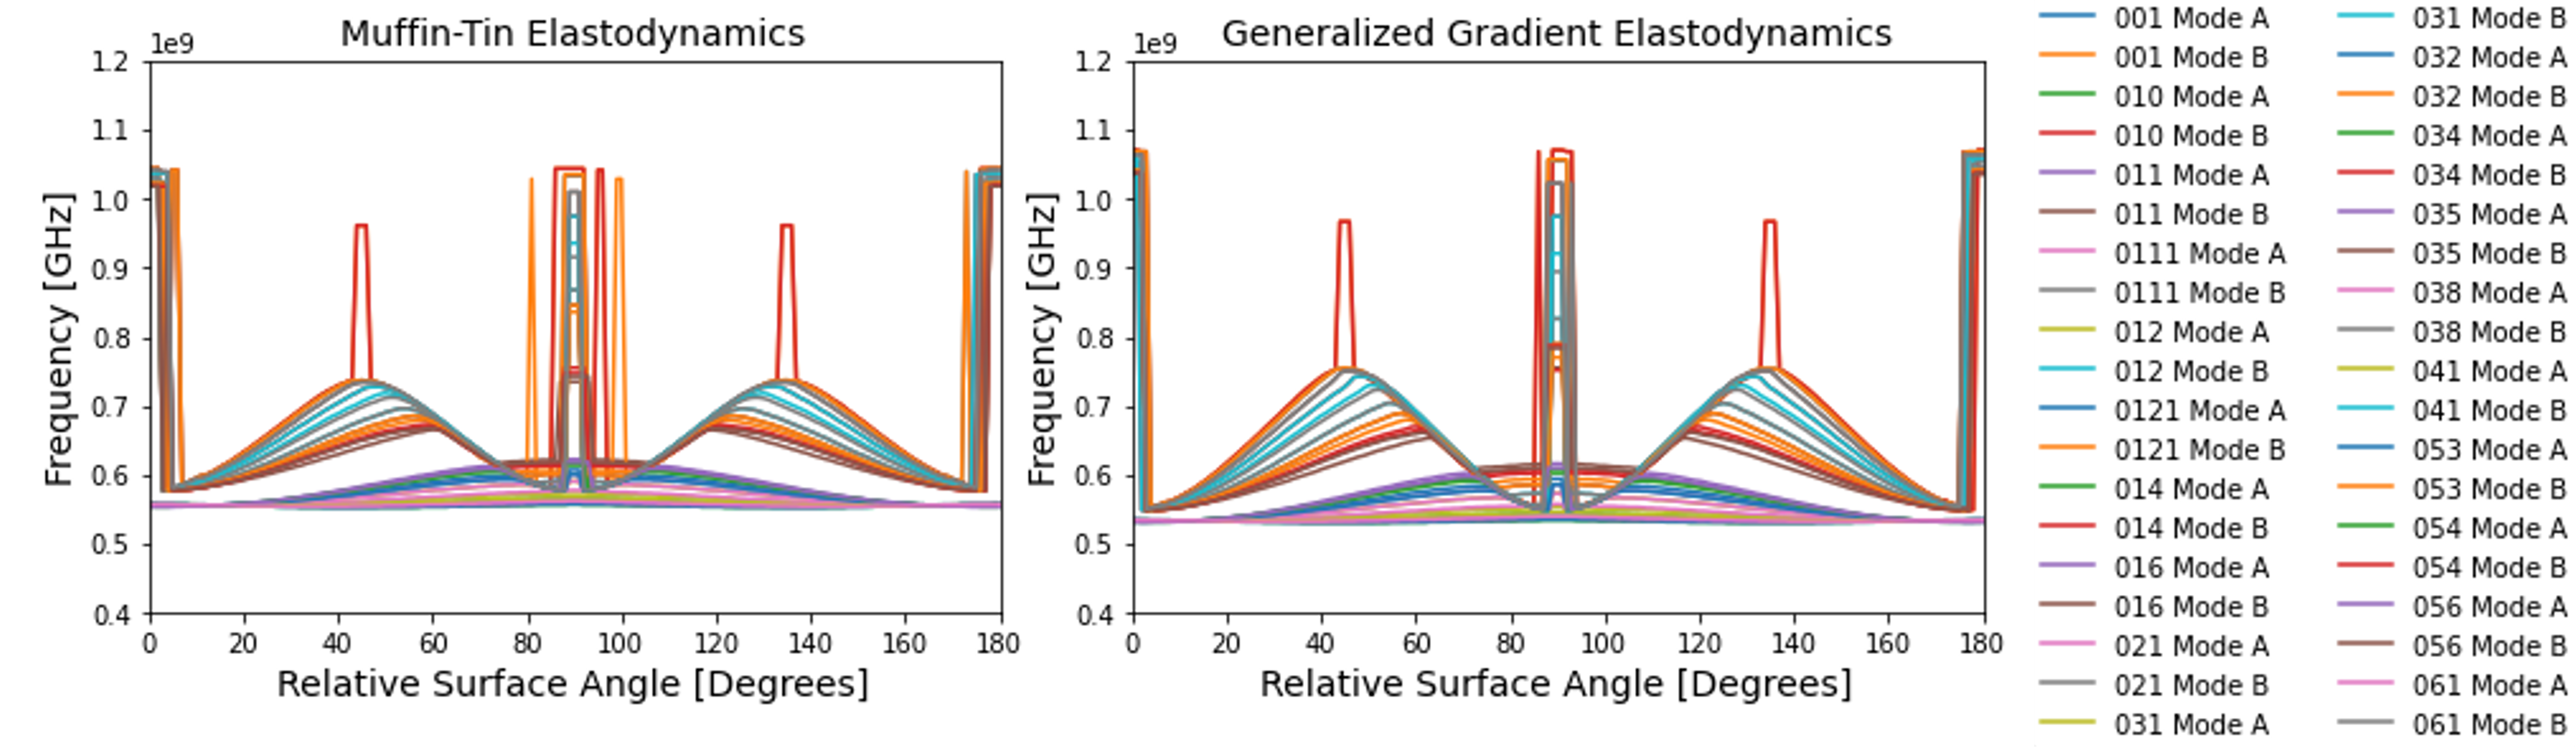
\includegraphics[width=\textwidth]{Parts/Figures/smoking-gun-v2.png}
        \caption{Predicted elastic frequencies showcasing the emergence of new modes within the elastodynamically-unallowed regions, signifying alterations in the material's mechanical properties due to spinodal decomposition. These frequencies match closely with experimentally observed values in aged stainless steel specimens, providing a quantum mechanical insight into the microstructural evolution impacting material performance.}
        \label{fig4a}
    \end{subfigure}
    \begin{subfigure}{0.35\textwidth}
        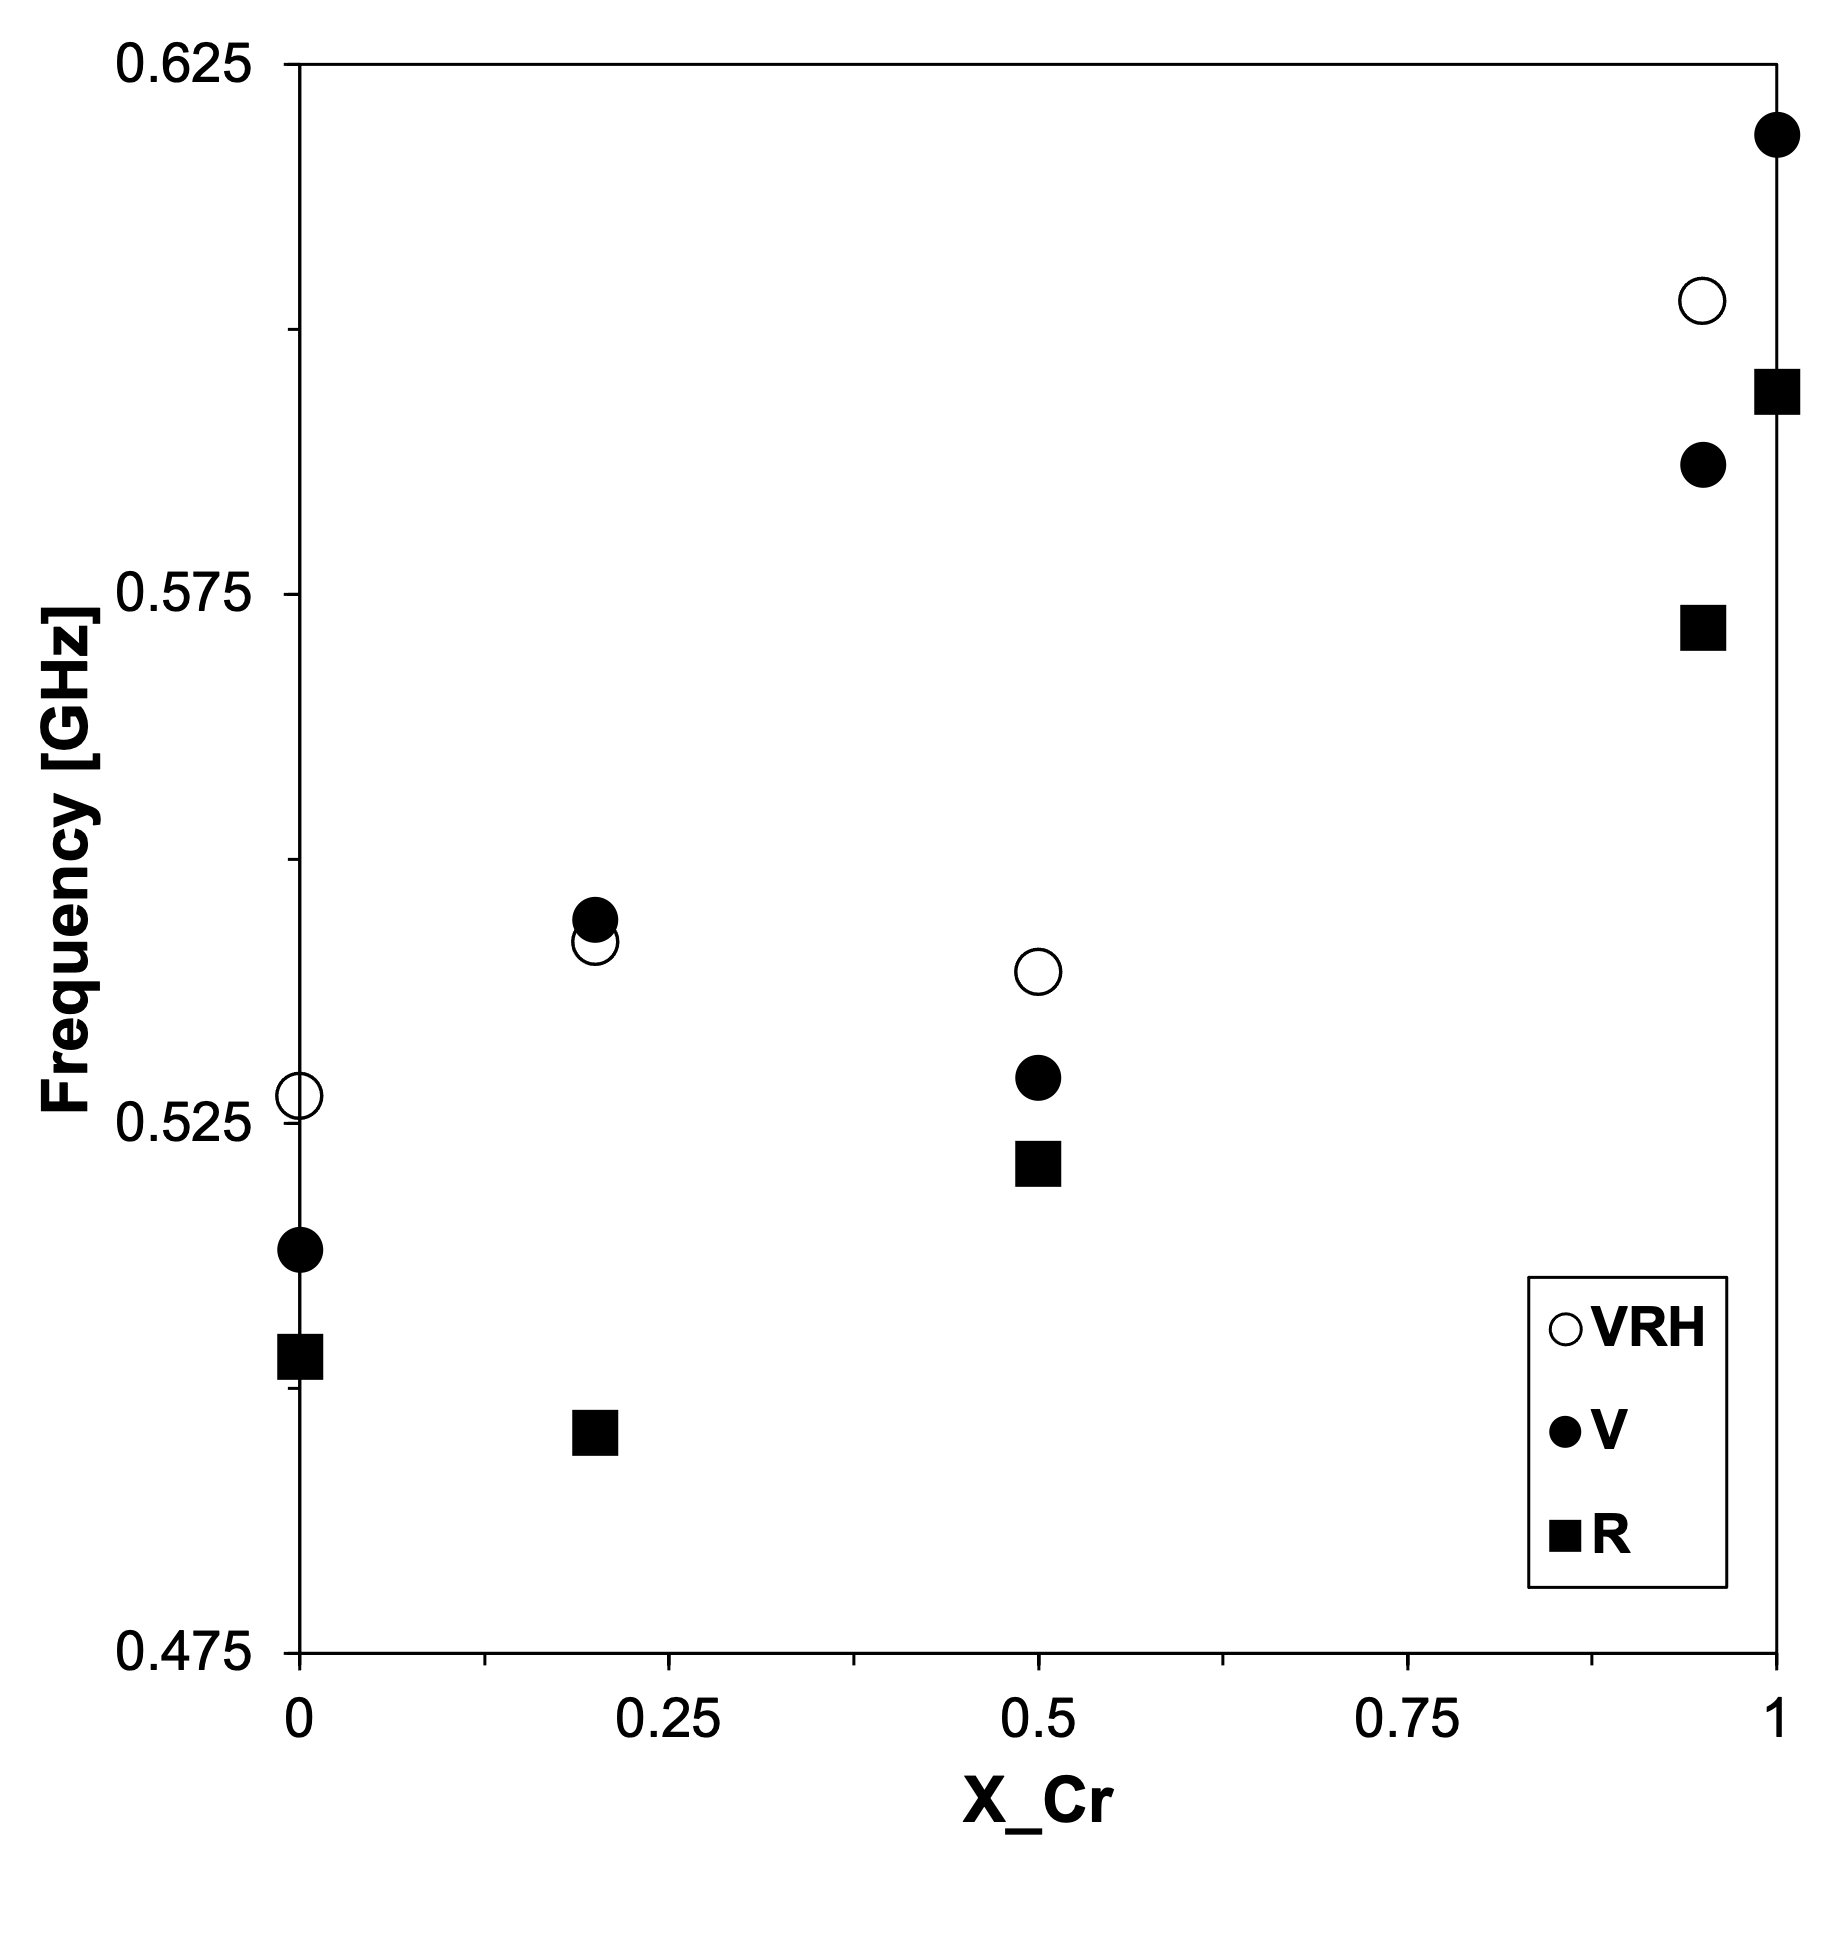
\includegraphics[width=\textwidth, left]{Parts/Figures/fvsX_v3.png}
        \caption{Calculated acoustic frequencies across different Cr compositions, illustrating the material's acoustic response variability with composition. This graph provides a quantitative measure of the material's mechanical behavior and its dependence on the microstructural characteristics induced by varying chromium content.}
        \label{fig4b}
    \end{subfigure}
    \begin{subfigure}{0.5\textwidth}
        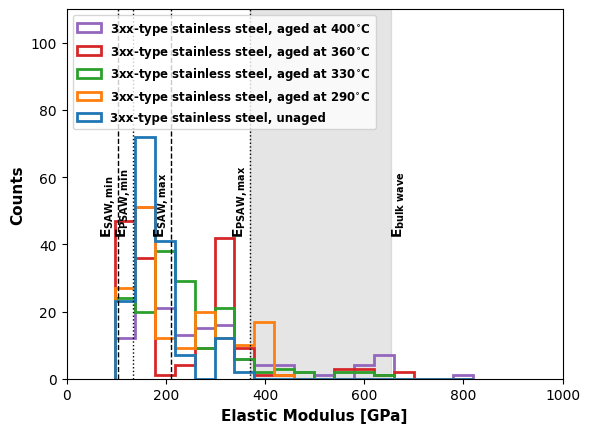
\includegraphics[width=\textwidth, right]{Parts/Figures/experimental-moduli-hist.png}
        \caption{Measured elastic moduli distribution from experimental data, highlighting the range and variability of material properties within stainless steel samples subjected to different thermal aging processes. The distribution underscores the significant impact of microstructural changes, such as spinodal decomposition, on the material's overall stiffness and mechanical integrity.}
        \label{fig4c}
    \end{subfigure}
    \caption{(a) Quantum elastodynamic frequencies obtained from density functional theory calculations reveal the complex interplay between microstructural evolution and mechanical properties in stainless steels undergoing spinodal decomposition. These findings are corroborated by (b) calculated acoustic frequencies that vary with Cr composition, providing a link between composition, microstructure, and acoustic properties. (c) The distribution of measured elastic moduli further validates the theoretical predictions, illustrating the broad impact of aging and compositional changes on the material's mechanical performance.}
    \label{fig4}
\end{sidewaysfigure}


\begin{sidewaysfigure}[!ht]
	\centering
	\begin{subfigure}{0.3\textwidth}
         \centering
         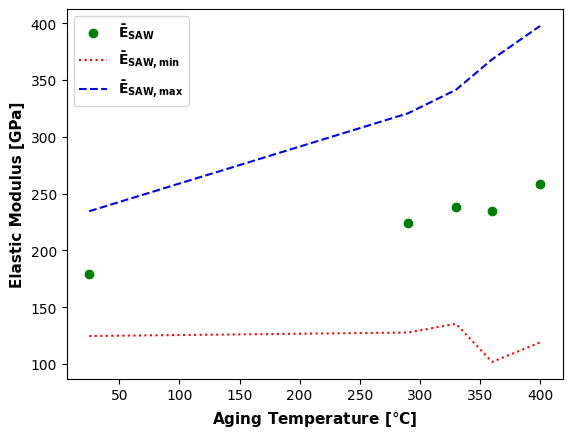
\includegraphics[width=\linewidth]{Parts/Figures/experimental-moduli-trend.png}
         \caption{Experimental elastic moduli of aged steels, displaying how aging temperature influences the material's stiffness. This graph illustrates the correlation between thermal treatment and the increase in elastic moduli, indicative of the material's response to microstructural changes over time.}
         \label{fig5a}
     \end{subfigure}
     \hfill
     \begin{subfigure}{0.3\textwidth}
         \centering
         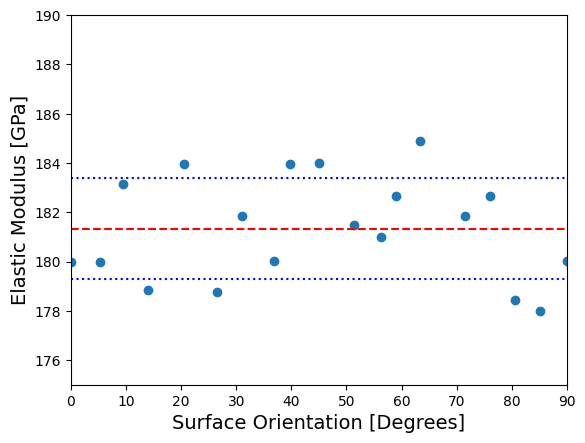
\includegraphics[width=\linewidth]{Parts/Figures/approximate-elastic-moduli-from-SAW-measurements-pristine.png}
         \caption{Theoretical elastic moduli of pristine steels, offering a baseline comparison for understanding how spinodal decomposition affects material properties before and after aging. This comparison elucidates the stiffening effect of microstructural evolution on the alloy's mechanical behavior.}
         \label{fig5b}
     \end{subfigure}
     \hfill
     \begin{subfigure}{0.3\textwidth}
         \centering
         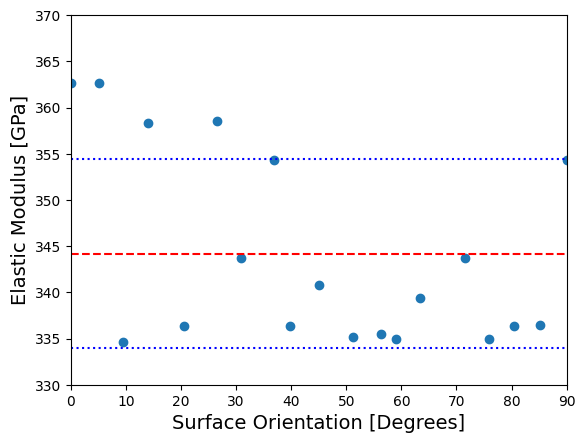
\includegraphics[width=\linewidth]{Parts/Figures/approximate-elastic-moduli-from-SAW-measurements-spindec.png}
         \caption{Theoretical elastic moduli of spinodally decomposed steels, demonstrating the pronounced impact of microstructural evolution on the alloy's stiffness. This direct comparison to pristine conditions highlights the significant role of chromium composition and thermal aging in material performance.}
         \label{fig5c}
     \end{subfigure}
     \hfill
     \begin{subfigure}{0.3\textwidth}
         \centering
         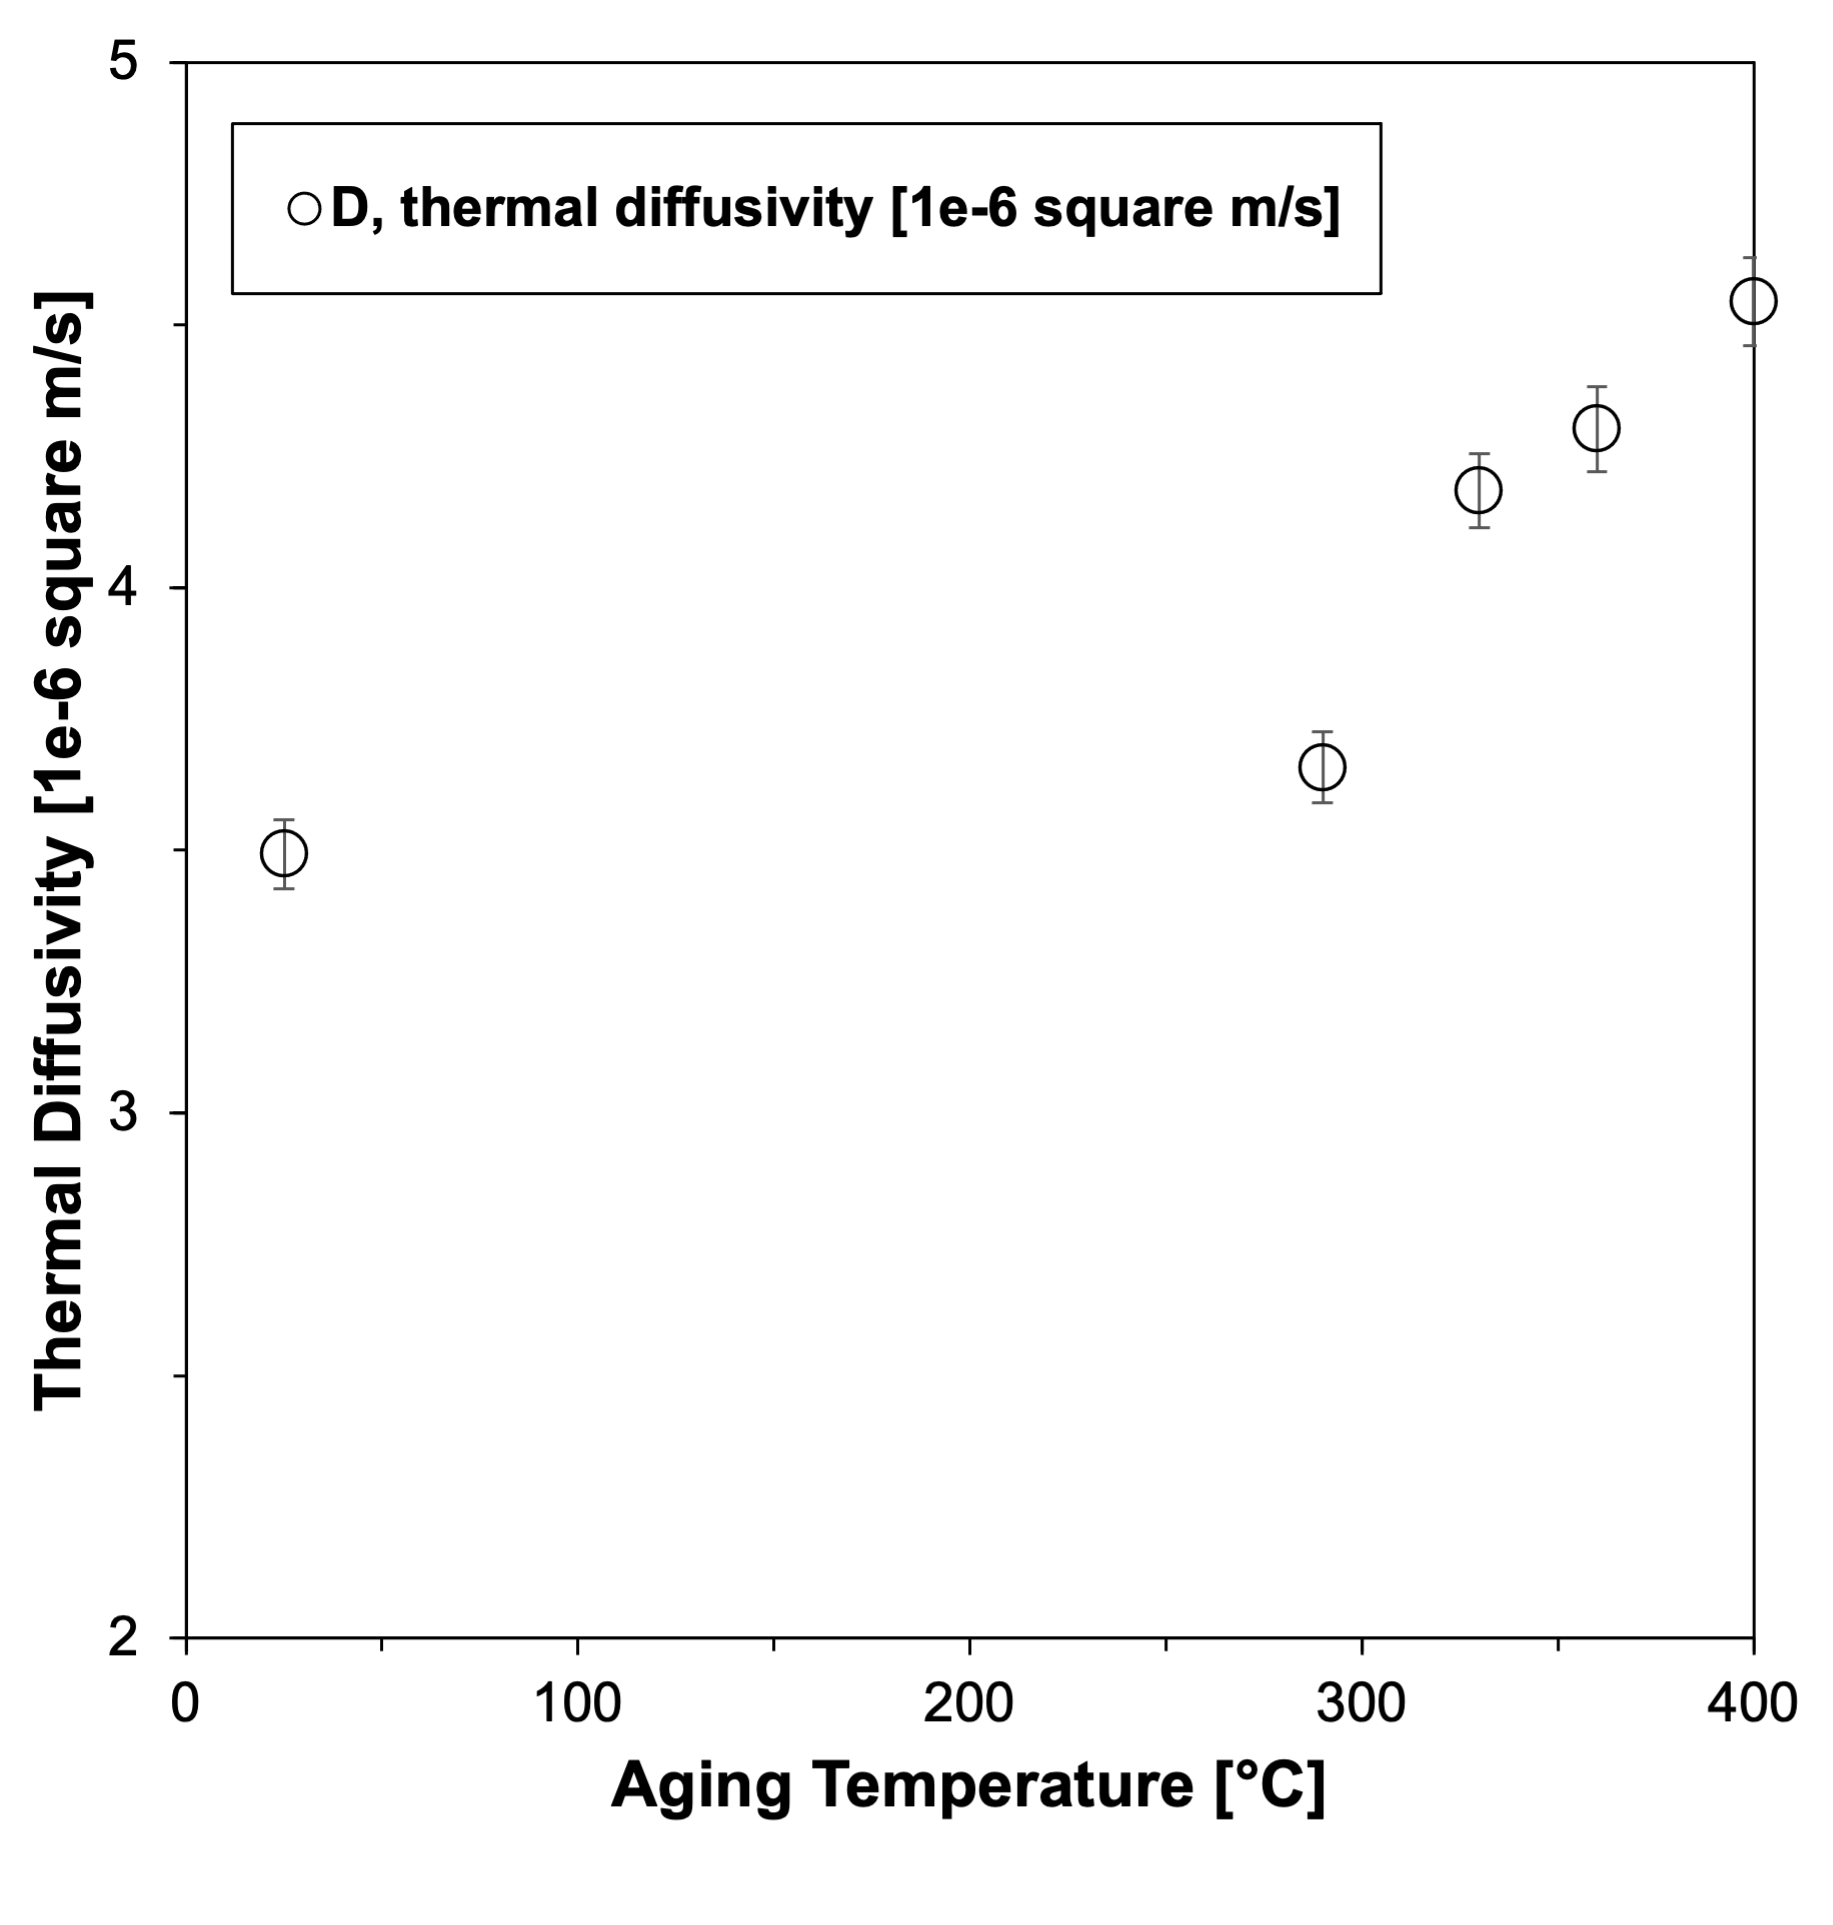
\includegraphics[width=\linewidth]{Parts/Figures/DvsT_CF8_30khrs_v2.png}
         \caption{\(D^{exp}_{thermal}\), experimental thermal diffusivity as measured in aged stainless steel, illustrating the thermal transport characteristics and their variation with temperature. This metric provides insights into the thermal stability and heat dissipation capabilities of the material post-aging.}
         \label{fig5d}
     \end{subfigure}
     \hfill
     \begin{subfigure}{0.3\textwidth}
         \centering
         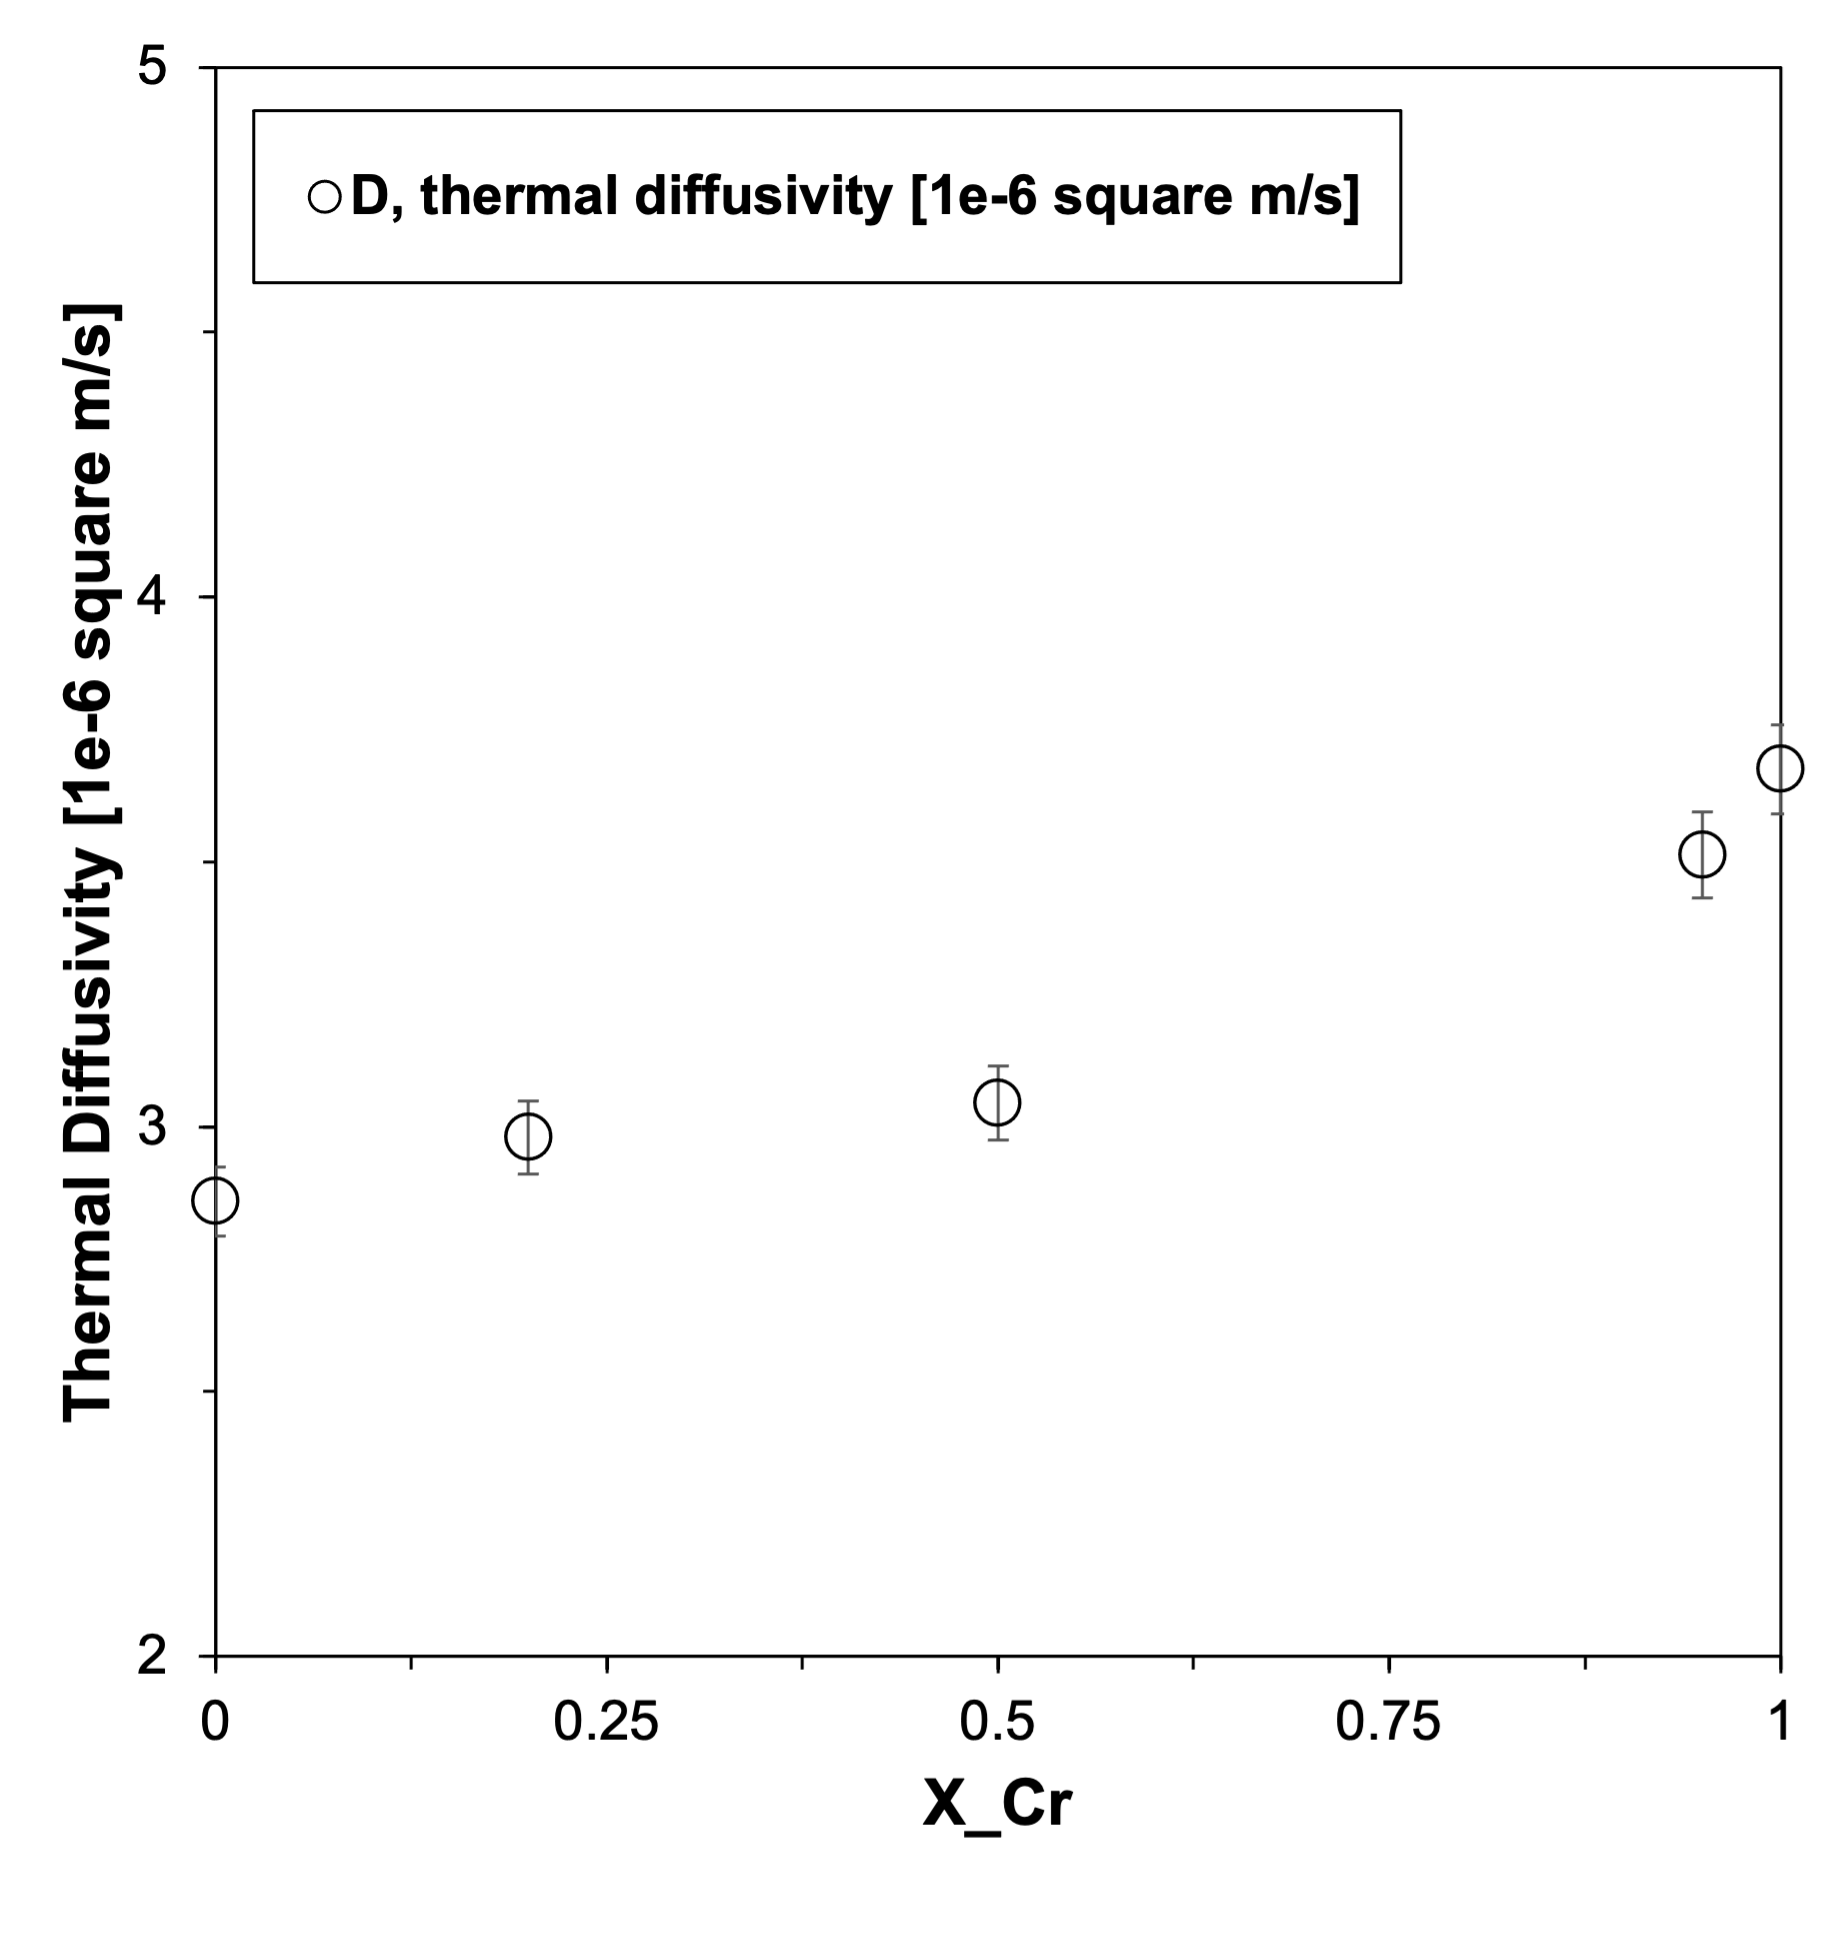
\includegraphics[width=\linewidth]{Parts/Figures/DvsX_v4.png}
         \caption{\(D^{theoretical}_{thermal}\), theoretical thermal diffusivity indicating the expected thermal behavior based on composition and microstructural considerations. This predictive analysis aids in understanding the thermal management potential of the alloy across a range of compositions.}
         \label{fig5e}
     \end{subfigure}
     \hfill
     \begin{subfigure}{0.3\textwidth}
         \centering
         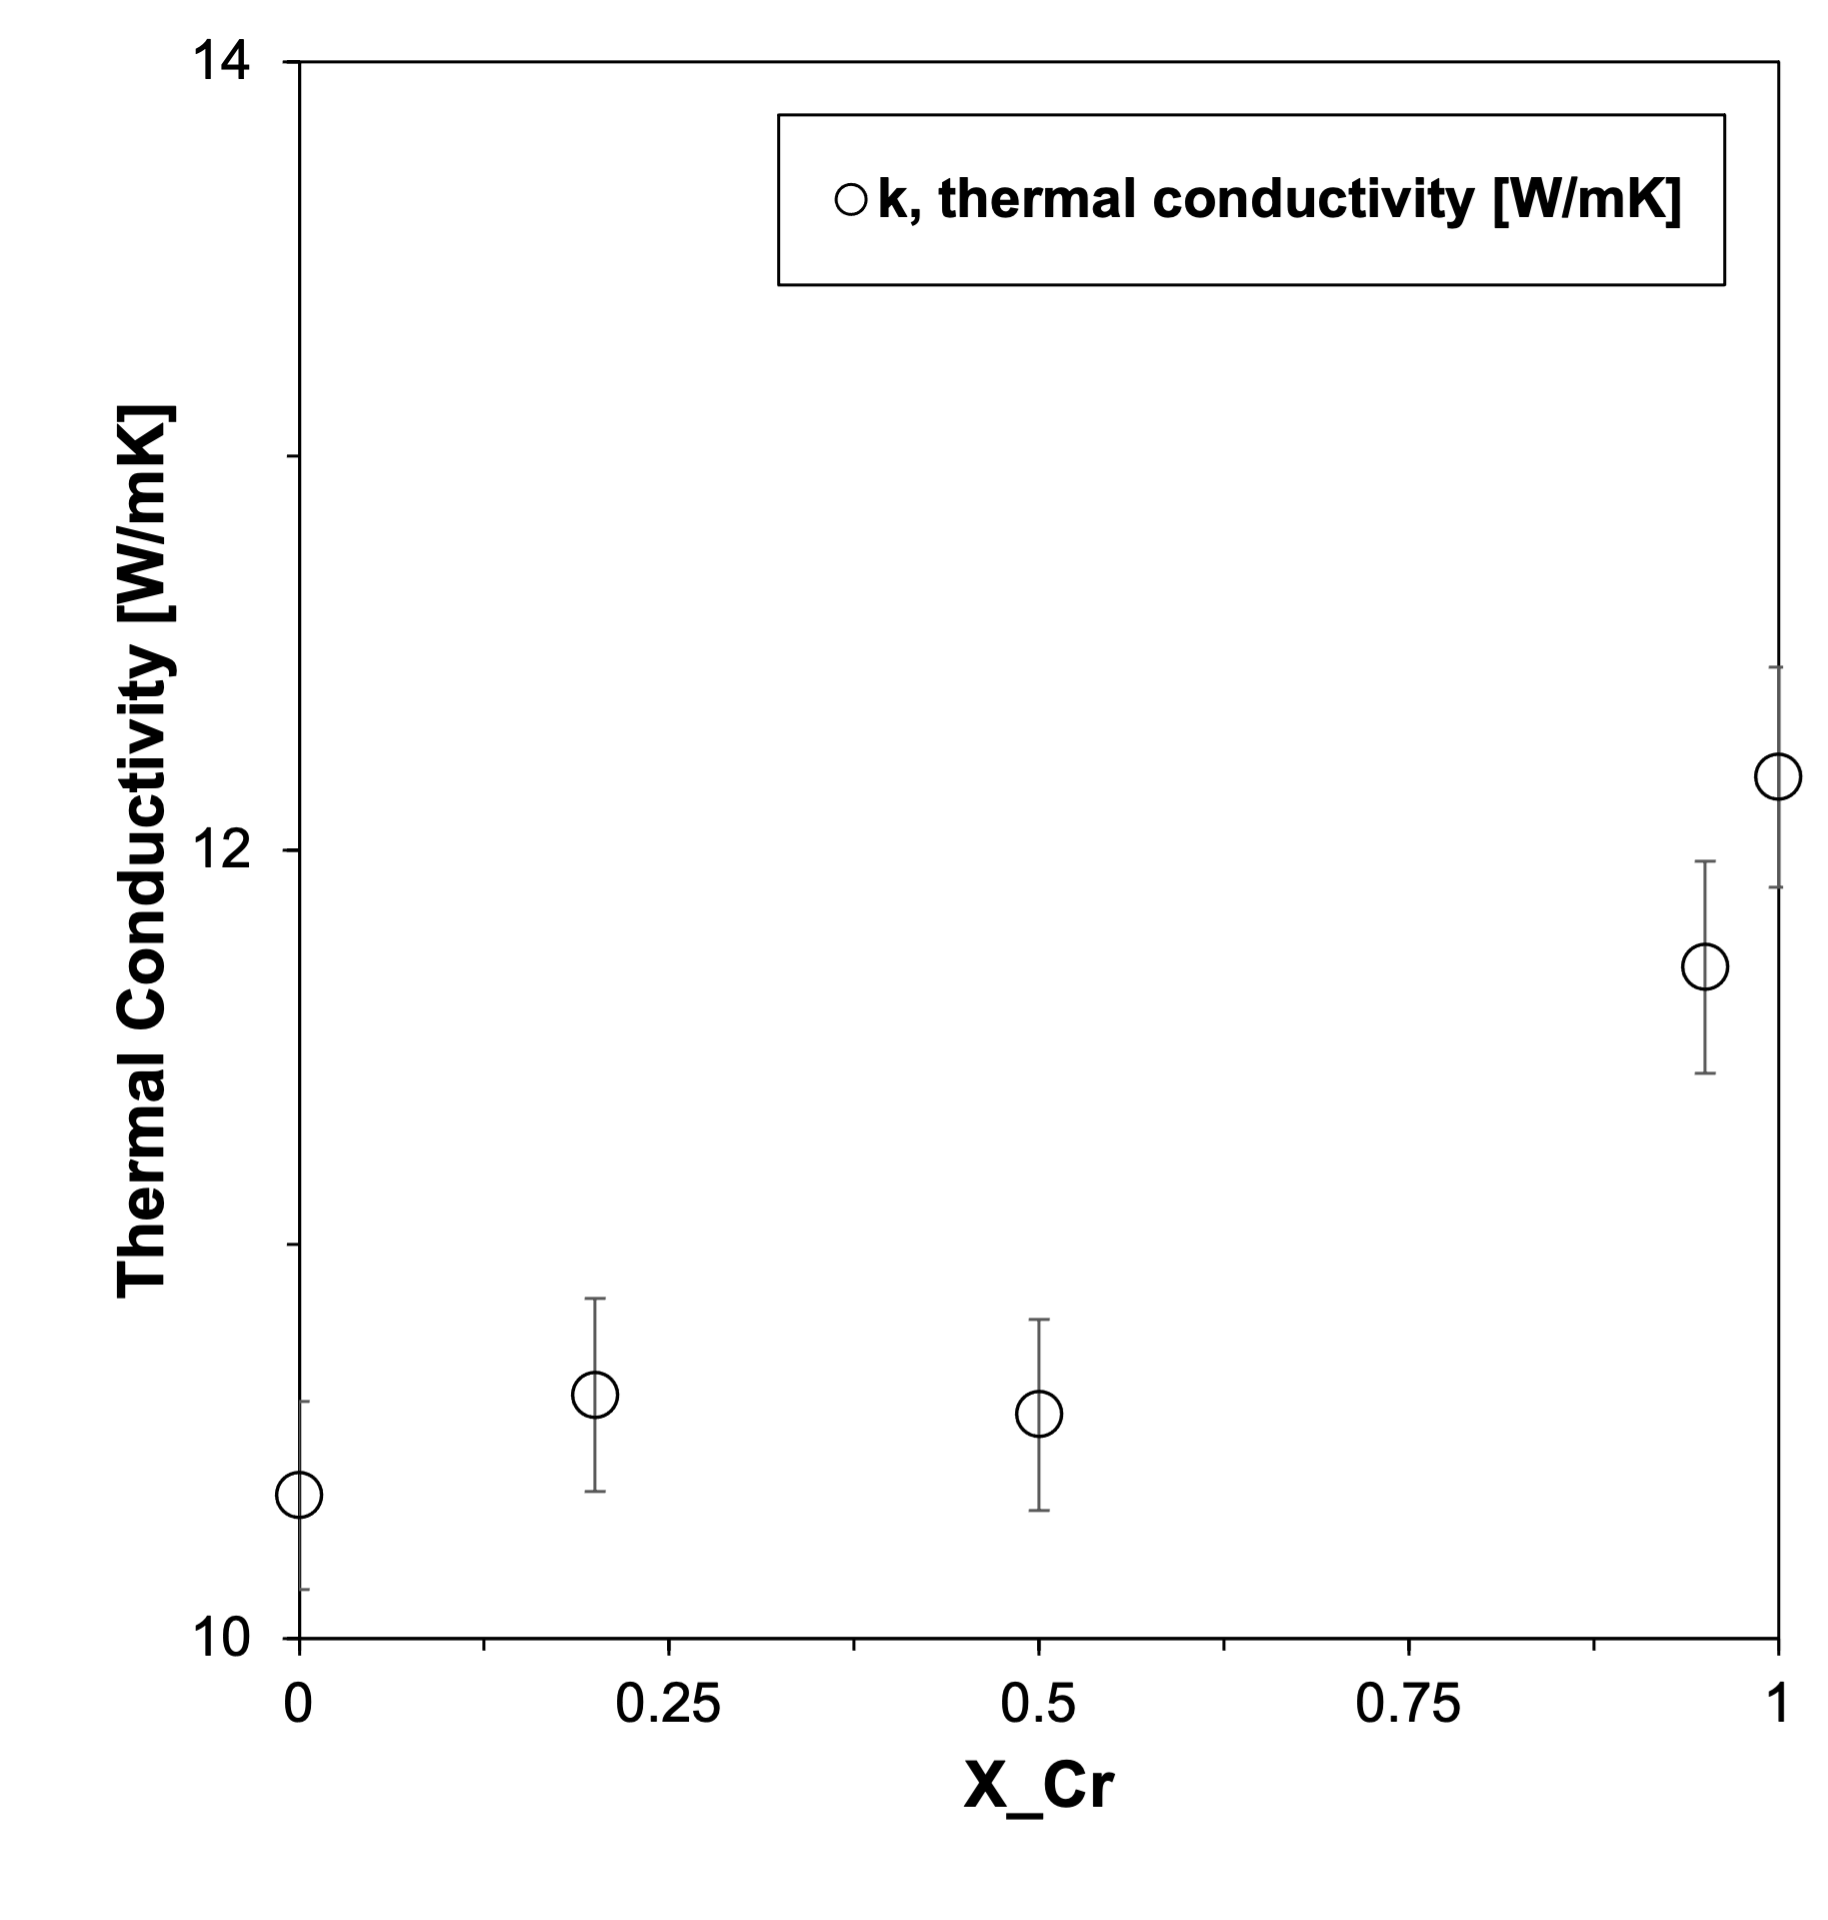
\includegraphics[width=\linewidth]{Parts/Figures/KvsX_v2.png}
         \caption{\(\kappa^{theoretical}_{thermal}\), thermal conductivity, showcasing the theoretical prediction of how efficiently the material conducts heat. This property is crucial for applications where thermal management is key, and it is influenced by the alloy's microstructure and composition.}
         \label{fig5f}
     \end{subfigure}
	\caption{Comprehensive analysis combining experimental and theoretical insights into the thermal and mechanical properties of stainless steels subjected to thermal aging. (a) Experimental elastic moduli trends with aging temperature highlight the stiffening effect of microstructural evolution. (b) and (c) Theoretical predictions for pristine and spinodally decomposed steels provide a comparative framework for assessing the impact of spinodal decomposition on material properties. (d) Experimental thermal diffusivity measurements, alongside (e) theoretical predictions for thermal diffusivity and (f) thermal conductivity, offer a holistic view of the material's thermal and mechanical behavior post-aging, emphasizing the interconnectedness of thermal properties, mechanical performance, and microstructural characteristics.}
	\label{fig5}
\end{sidewaysfigure}
